\chapter{Experimental analysis}
\label{chapter:results-analysis}

In this chapter we analyse the results produced by the four models developed in this thesis. We are going to compare their outputs for each of the three problems considered: free elastica, constrained elastica and image segmentation.~\cref{ch9:tab:models-summary} summarizes the models properties.

In the image segmentation section, we compare our results with the linear model for curvature regularization of~\cite{schoenemann09linear}.

\begin{table}[H]
\footnotesize
\centering
\begin{tabular}{r|ccccc}
\multirow{2}{*}{Model} & \multirow{2}{*}{Implementation} & Running & Free  & Constrained & Image\\
& & Time & Elastica & Elastica & Segmentation\\
\hline
LocalSearch (LS) & medium & slow & yes(opt) & yes & no \\
FlipFlow (FF) & hard & acceptable & yes & no & yes \\
BalanceFlow (BF) & medium & acceptable & yes & no & yes \\
GraphFlow (GF) & easy & fast & yes(opt) & yes & yes
\end{tabular}
\caption{\daniel{\textbf{Models summary.}} The qualitative attributes are relative, e.g., the GraphFlow presents the lowest running time while LocalSearch presents the highest.}
\label{ch9:tab:models-summary}
\end{table}

\section{Free elastica}

The free elastica problem consists in finding a shape with the lowest digital elastica. The approach to solve this problem, as well the two others that follow, is to iteratively evolve an initial shape to another with lower digital elastica value. We have ran two experiments, summarized in~\cref{ch9:tab:free-elastica-parameters-summary}, to illustrate the evolution process behavior for each of the models described in this thesis. 

We make a distinction between the radius used to compute the balance coefficient $(bRadius)$ and the one used to estimate curvature using the II-estimator $(vRadius)$ in the validation function of GraphFlow and LocalSearch. In particular, the $vRadius$ is the one used to plot the graphs in~\cref{ch9:fig:plots-free-elastica-general,ch9:fig:plots-free-elastica-radius-choice}. Moreover, the $vRadius$ is always scaled by the grid step, while the $bRadius$ is never scaled.

\begin{table}
\centering
\begin{tabular}{|c|c|c|c|c|c|c|c|c|c|}
\cline{8-10}
\multicolumn{7}{c|}{} & FF,BF & \multicolumn{2}{|c|}{GF}\\
\hline
Experiment & $maxIt$ & $vRadius$ & $bRadius$ & $h$ & $\alpha$ & $\beta$  & $m$ & $a$ & $n$ \\
\hline
Exp-General & $400$ & $5$ & $7$ & $0.25$ & $0.01$ & $1$  & $5$ & $2$ & $3$ \\
\hline
\multirow{2}{*}{Exp-Radius} & \multirow{2}{*}{$400$} & \multirow{2}{*}{$5$} & $7$ & \multirow{2}{*}{$0.25$} &  \multirow{2}{*}{$0.001$} & \multirow{2}{*}{$1$}  & $5$ & \multirow{2}{*}{$2$} & \multirow{2}{*}{$3$} \\
& &  & $12$ & &  & & $10$ & &  \\
\hline
\end{tabular}
\caption{\daniel{\textbf{Parameter settings for the free elastica experiments.} The headers FF,BF,GF identifies specific parameters for the FlipFlow, BalanceFlow and GraphFlow models, respectively.}}
\label{ch9:tab:free-elastica-parameters-summary}
\end{table}

\subsection{Exp-General}

  The Exp-General experiment executes each model using the listed parameters in~\cref{ch9:tab:free-elastica-parameters-summary} for $5$ different parametric shapes. The results for the Exp-General experiment are shown in~\cref{ch9:fig:results-free-elastica-general}. One can check in the plots of~\cref{ch9:fig:plots-free-elastica-general} how the digital elastica value evolves at each iteration. For this experiment we also provide~\cref{ch9:tab:rtime-free-elastica-general} with the model's respective running times.
  

We observe that both LocalSearch and GraphFlow evolves the initial shape to another shape closer to the optimal one, e.g., for $\alpha=0.01$, the model evolves to the disk of radius $10$. However, the GraphFlow model is simpler to implement and much faster than LocalSearch (see~\cref{ch9:tab:rtime-free-elastica-general}). Even with a smaller neighborhood, the GraphFlow achieves its convergence before LocalSearch in two occasions, one in the square and another in the flower evolution.

At the first iterations, FlipFlow and BalanceFlow produce shapes with lower digital elastica energy. However, the models do not stop to evolve even if a shape of smaller perimeter and lower digital elastica ceases to exist, and starting from this point, the digital elastica value increases.


\begin{figure}
\center
\captionsetup{type=table}
\footnotesize
\begin{tabular}{|l|c|c|c|c|c|}
\hline
& Pixels (initial shape) & LocalSearch & FlipFlow & BalanceFlow & GraphFlow \\
\hline
Triangle & 8315 & 4.8s/it & 0.4s/it & 0.38s/it & 0.14s/it\\
Square & 12769 & 2s/it & 0.51s/it & 0.47s/it & 0.12s/it\\
Ellipse  & 10038 & 3.1s/it & 0.64s/it & 0.57s/it & 0.1s/it \\
Flower & 26321 & 12.3s/it & 1.23s/it & 0.94s/it & 0.14s/it\\
Bean  & 25130 & 6.4s/it & 1.2s/it & 1.17s/it & 0.16s/it\\
\hline
\end{tabular}
\caption{\daniel{\textbf{Exp-General summary.}} Running time and input size of Exp-General experiment for the free elastica.}
\label{ch9:tab:rtime-free-elastica-general} 
\end{figure}


\begin{figure}
\begin{tabular}{cccc}
LocalSearch & FlipFlow & BalanceFlow & GraphFlow\\[1em]
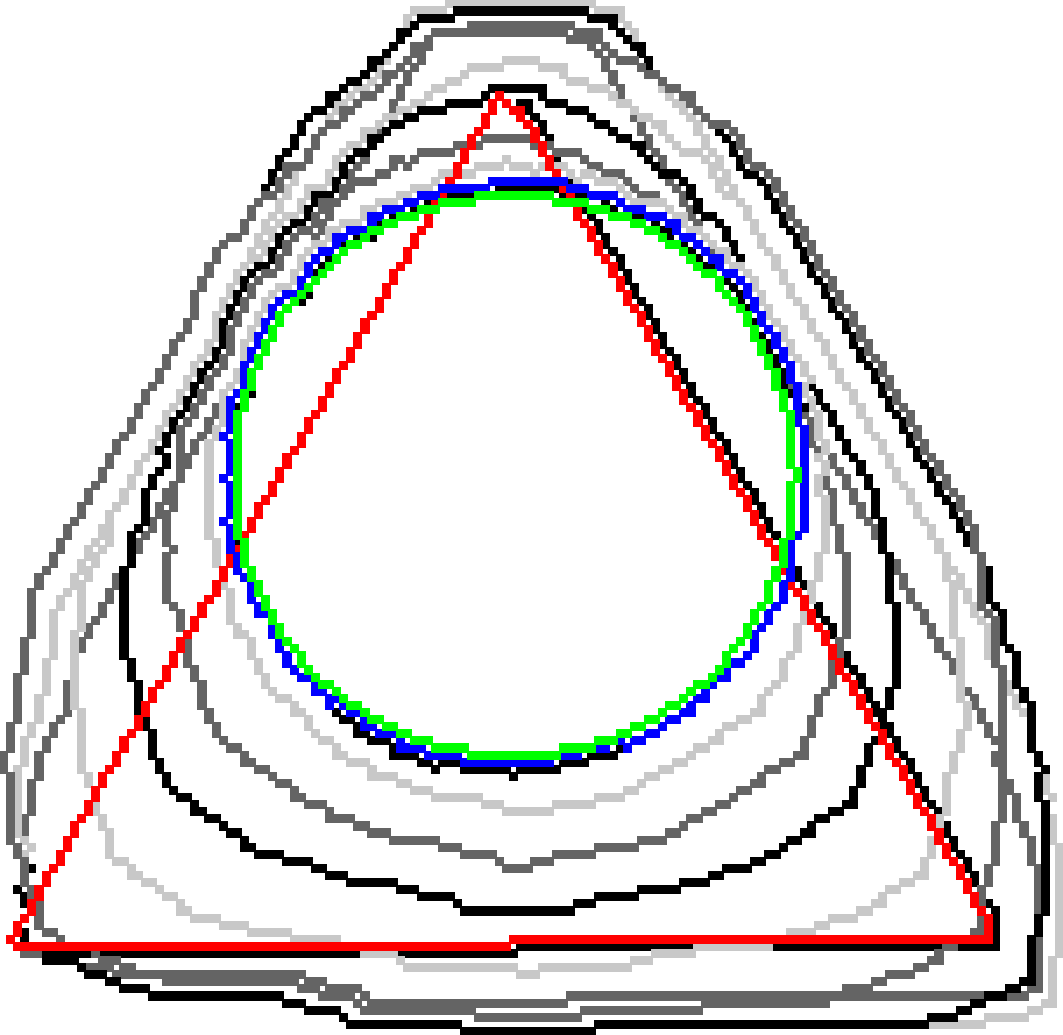
\includegraphics[scale=0.15]{figures/chapter9/free-elastica/localsearch/triangle/len_pen-0.01/radius-7/summary.pdf} & 
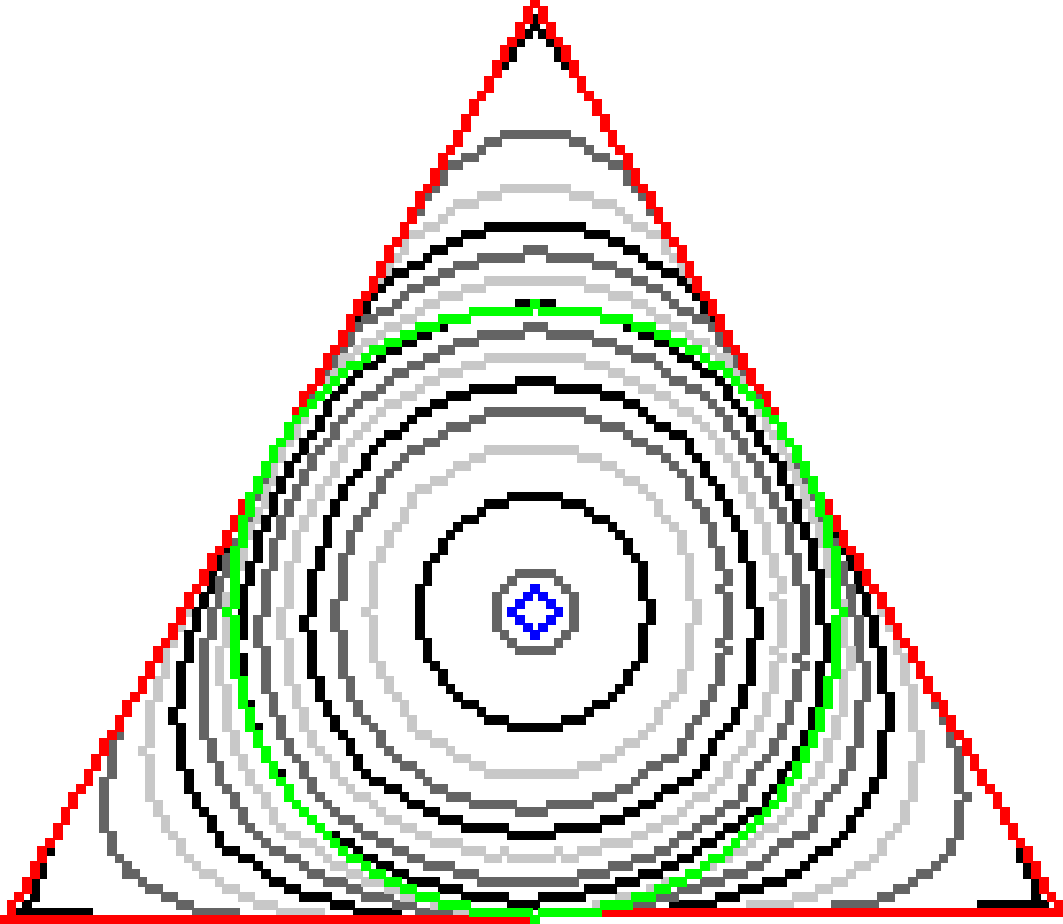
\includegraphics[scale=0.15]{figures/chapter9/free-elastica/flipflow/triangle/len_pen-0.01/radius-7/summary.pdf} &
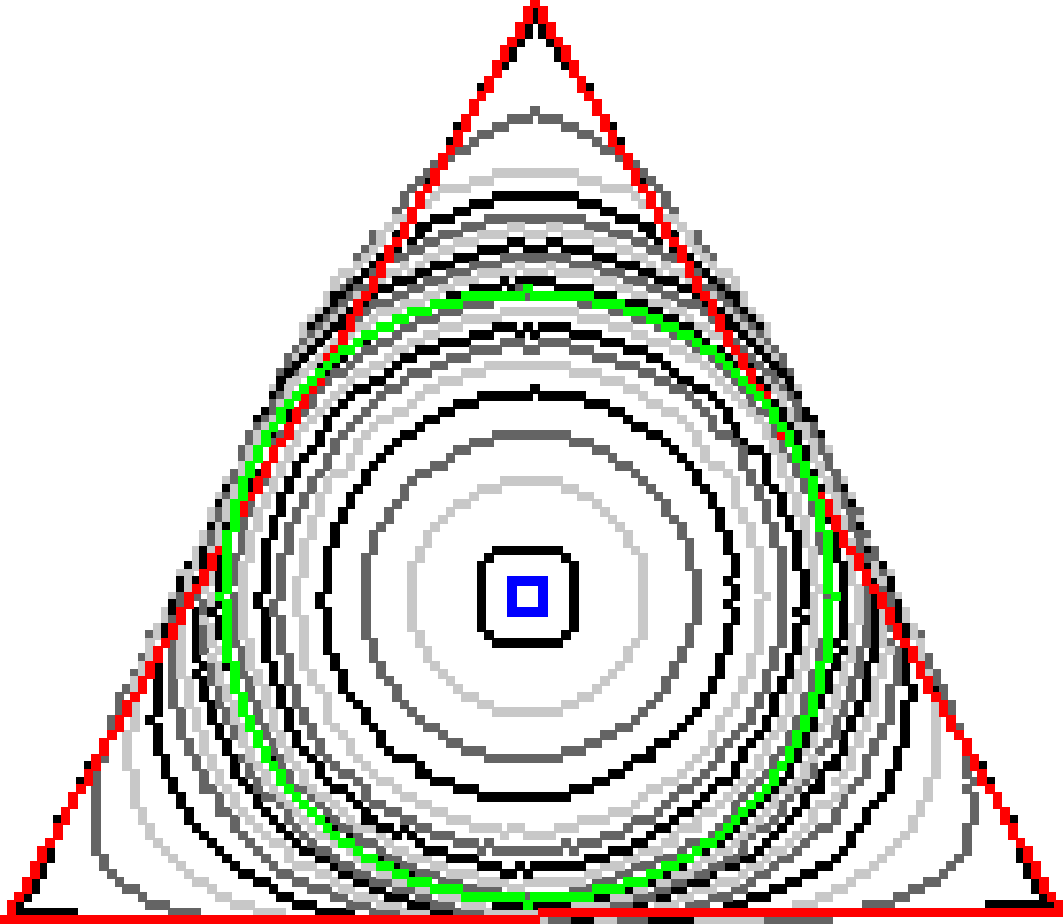
\includegraphics[scale=0.15]{figures/chapter9/free-elastica/balanceflow/triangle/len_pen-0.01/radius-7/summary.pdf} &
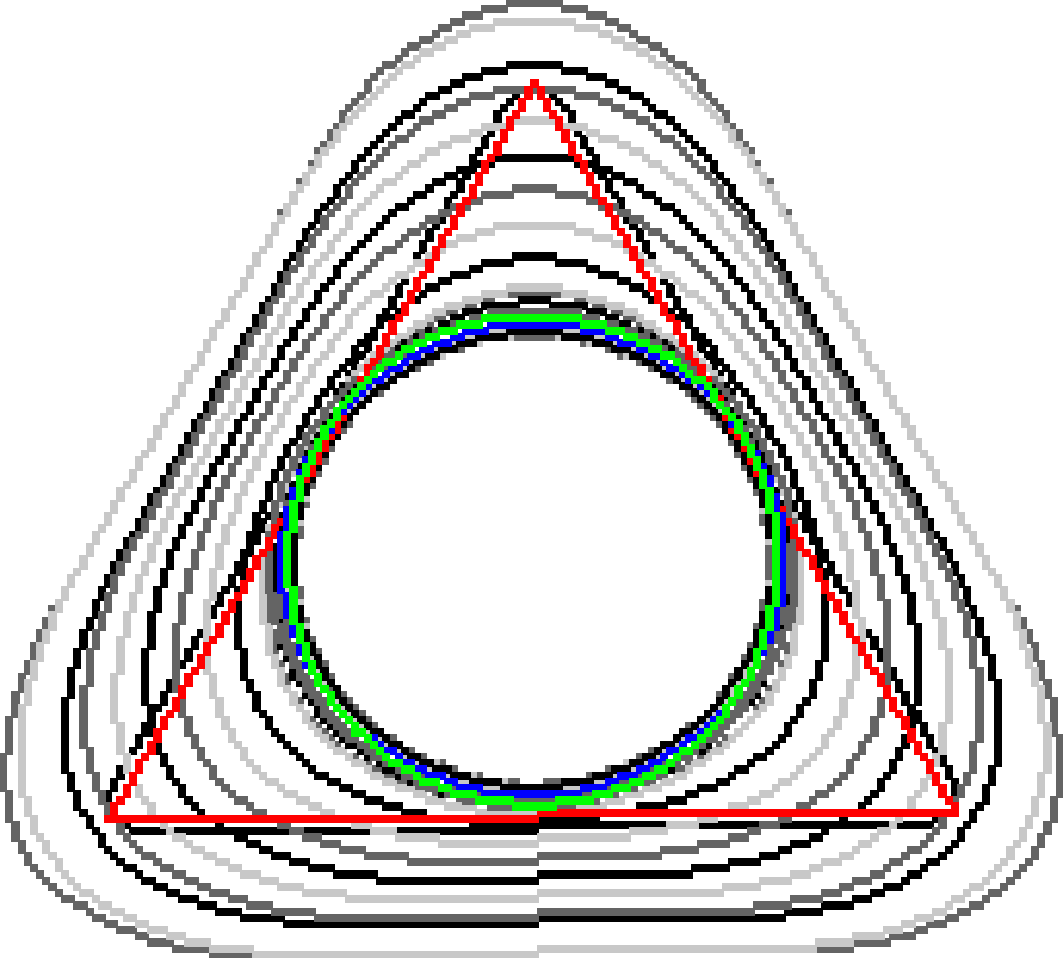
\includegraphics[scale=0.15]{figures/chapter9/free-elastica/graphflow/triangle/len_pen-0.01/radius-7/summary.pdf} \\[1em]
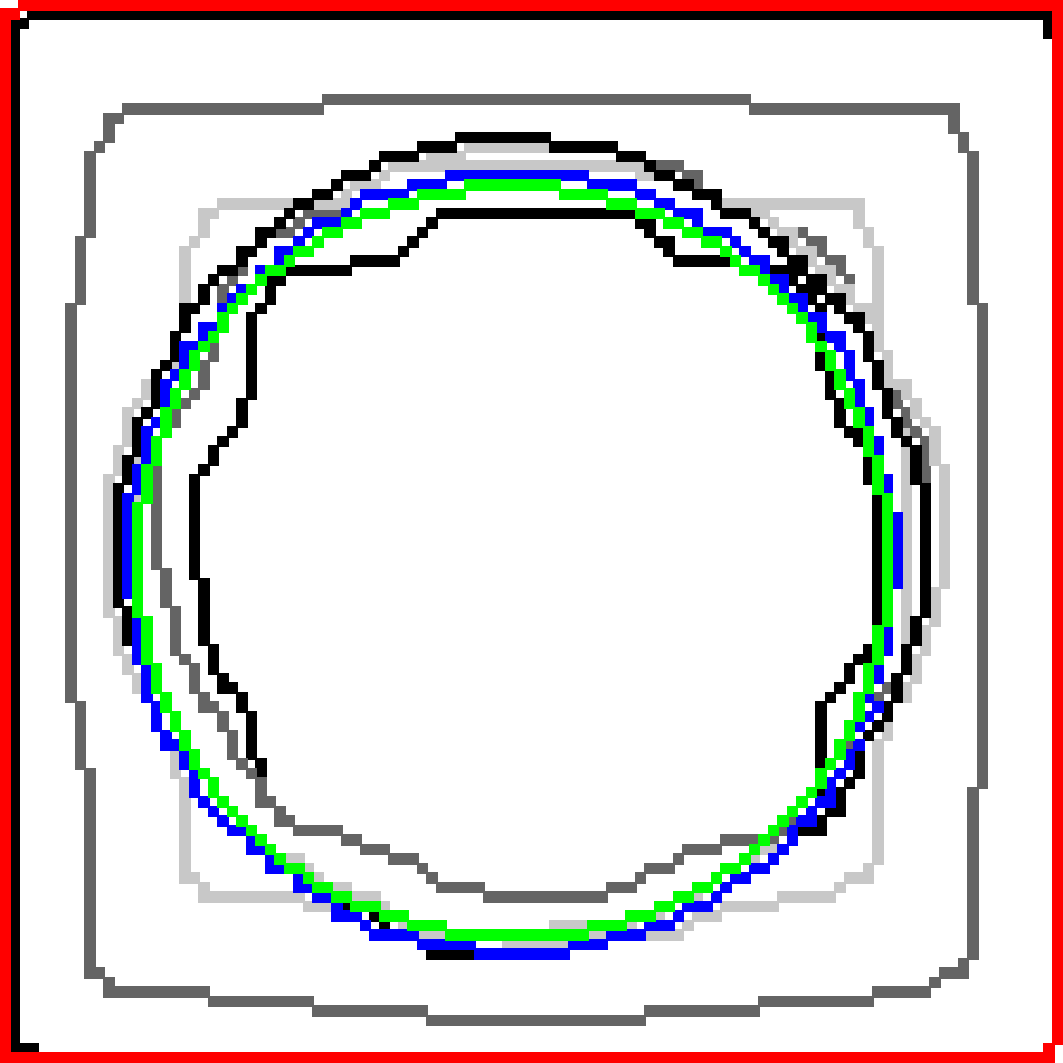
\includegraphics[scale=0.15]{figures/chapter9/free-elastica/localsearch/square/len_pen-0.01/radius-7/summary.pdf} & 
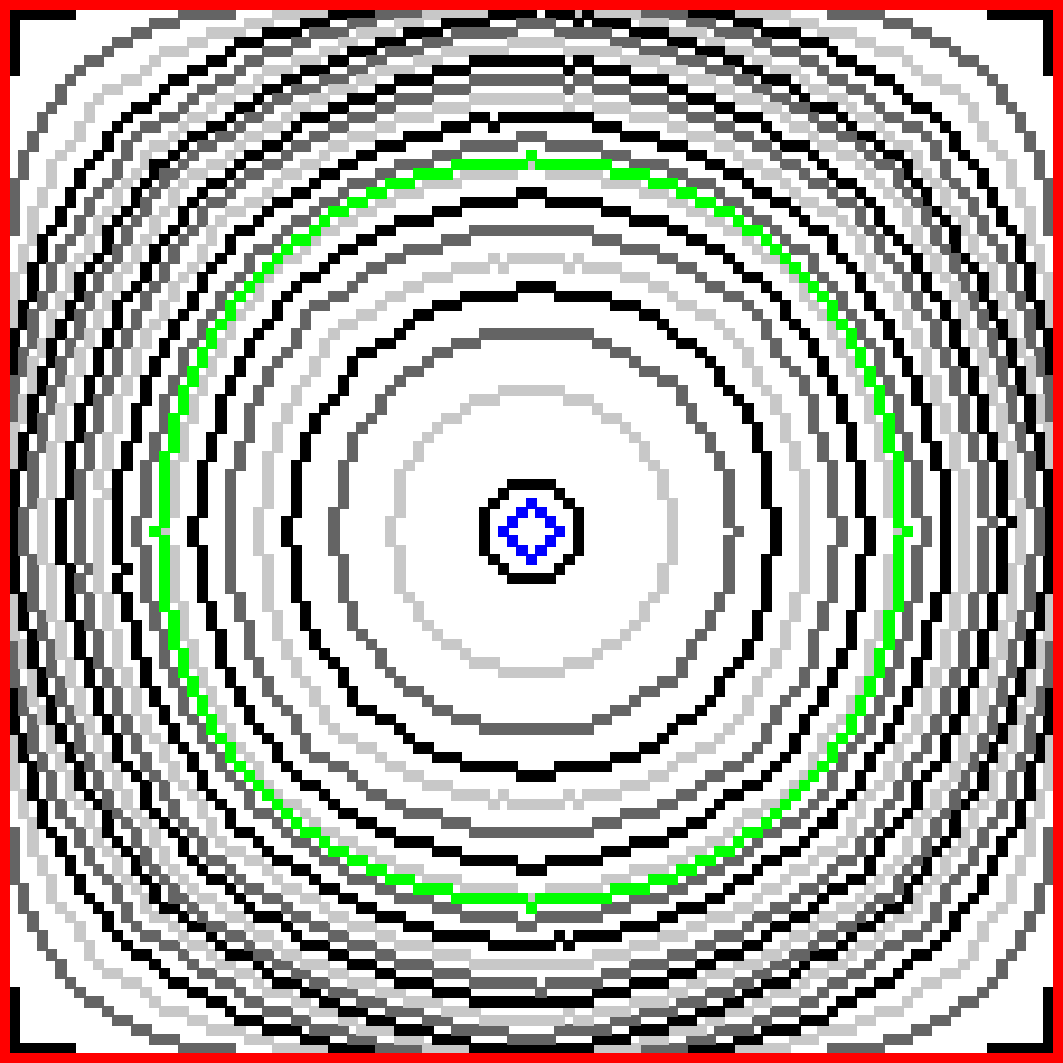
\includegraphics[scale=0.15]{figures/chapter9/free-elastica/flipflow/square/len_pen-0.01/radius-7/summary.pdf} &
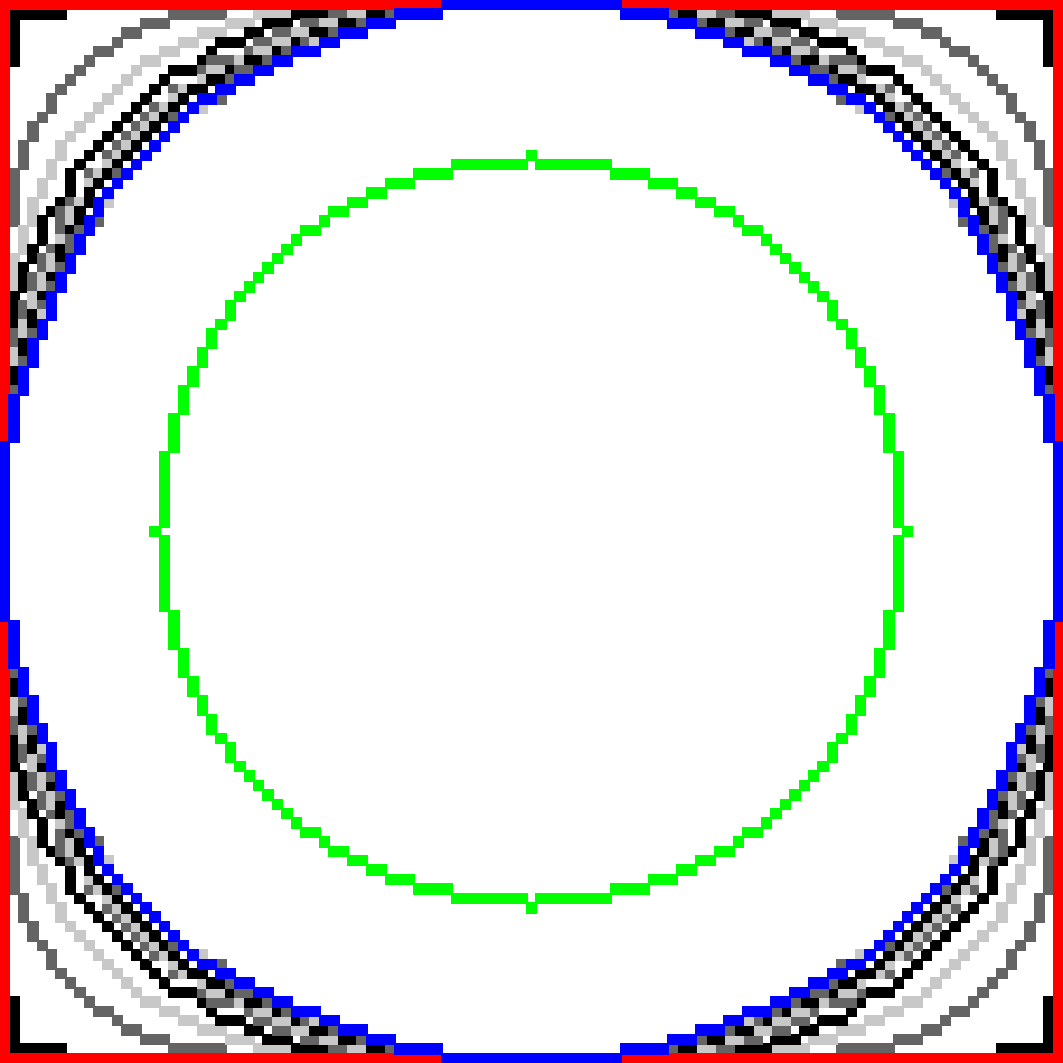
\includegraphics[scale=0.15]{figures/chapter9/free-elastica/balanceflow/square/len_pen-0.01/radius-7/summary.pdf} &
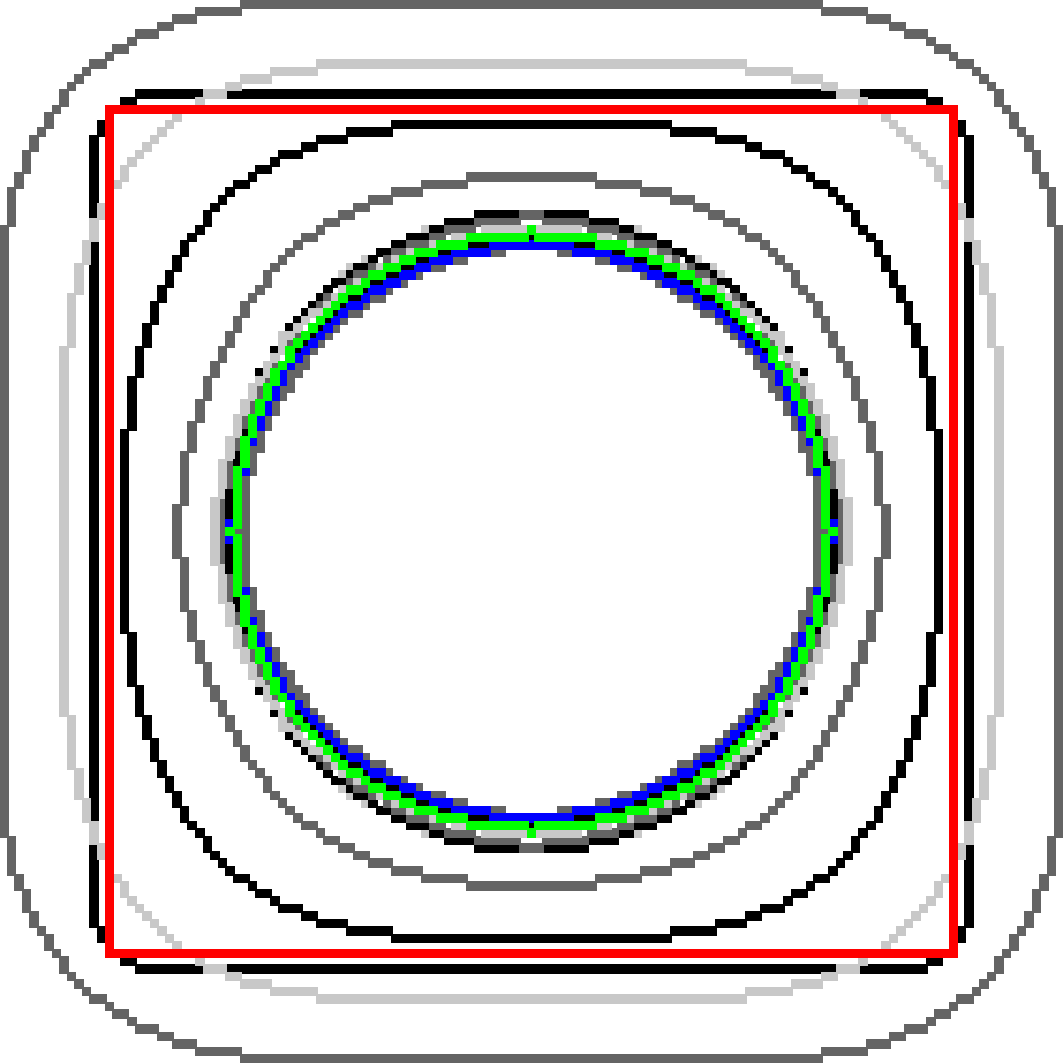
\includegraphics[scale=0.15]{figures/chapter9/free-elastica/graphflow/square/len_pen-0.01/radius-7/summary.pdf} \\[1em]
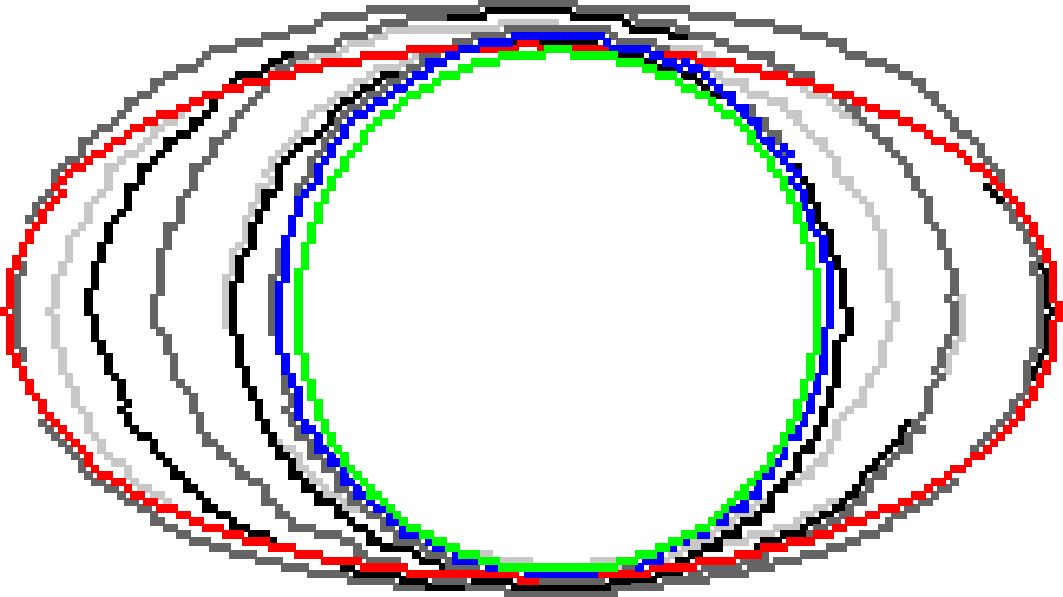
\includegraphics[scale=0.18]{figures/chapter9/free-elastica/localsearch/ellipse/len_pen-0.01/radius-7/summary.pdf} & 
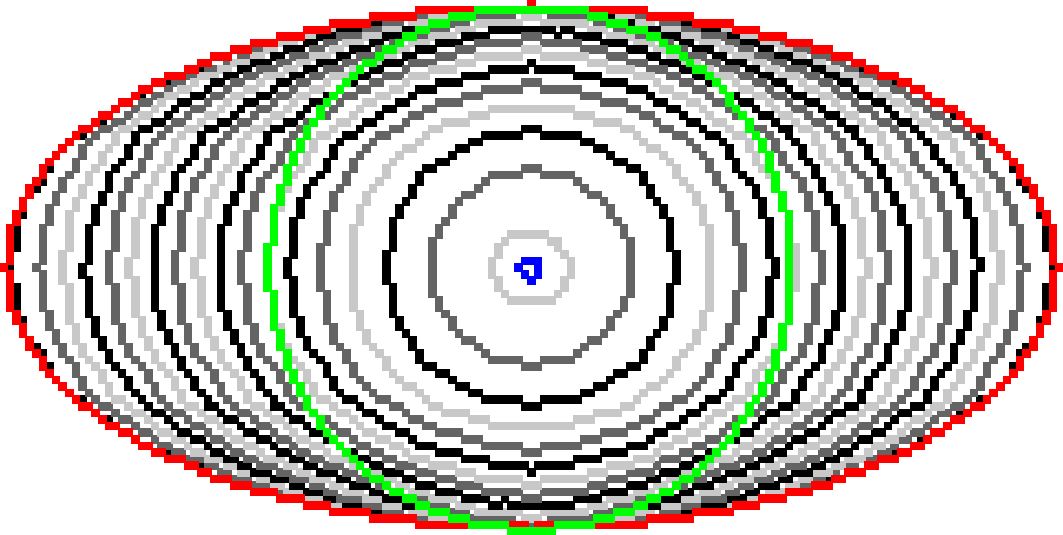
\includegraphics[scale=0.18]{figures/chapter9/free-elastica/flipflow/ellipse/len_pen-0.01/radius-7/summary.pdf} &
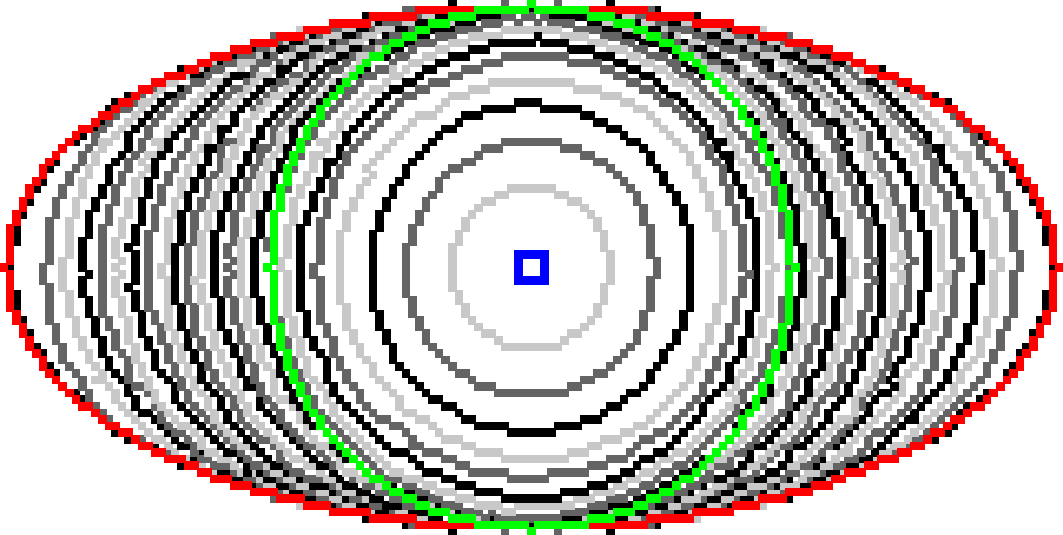
\includegraphics[scale=0.18]{figures/chapter9/free-elastica/balanceflow/ellipse/len_pen-0.01/radius-7/summary.pdf} &
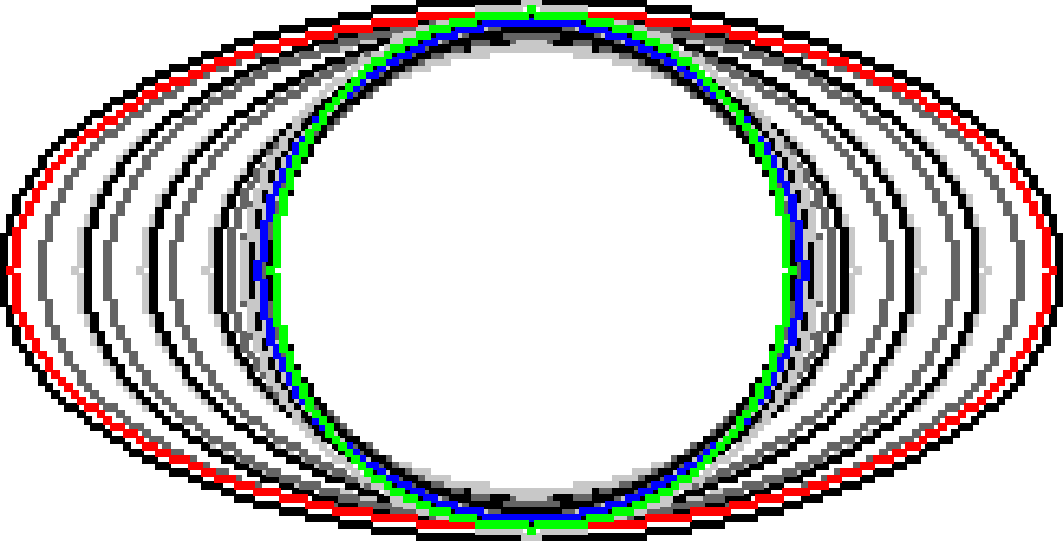
\includegraphics[scale=0.18]{figures/chapter9/free-elastica/graphflow/ellipse/len_pen-0.01/radius-7/summary.pdf} \\[1em]
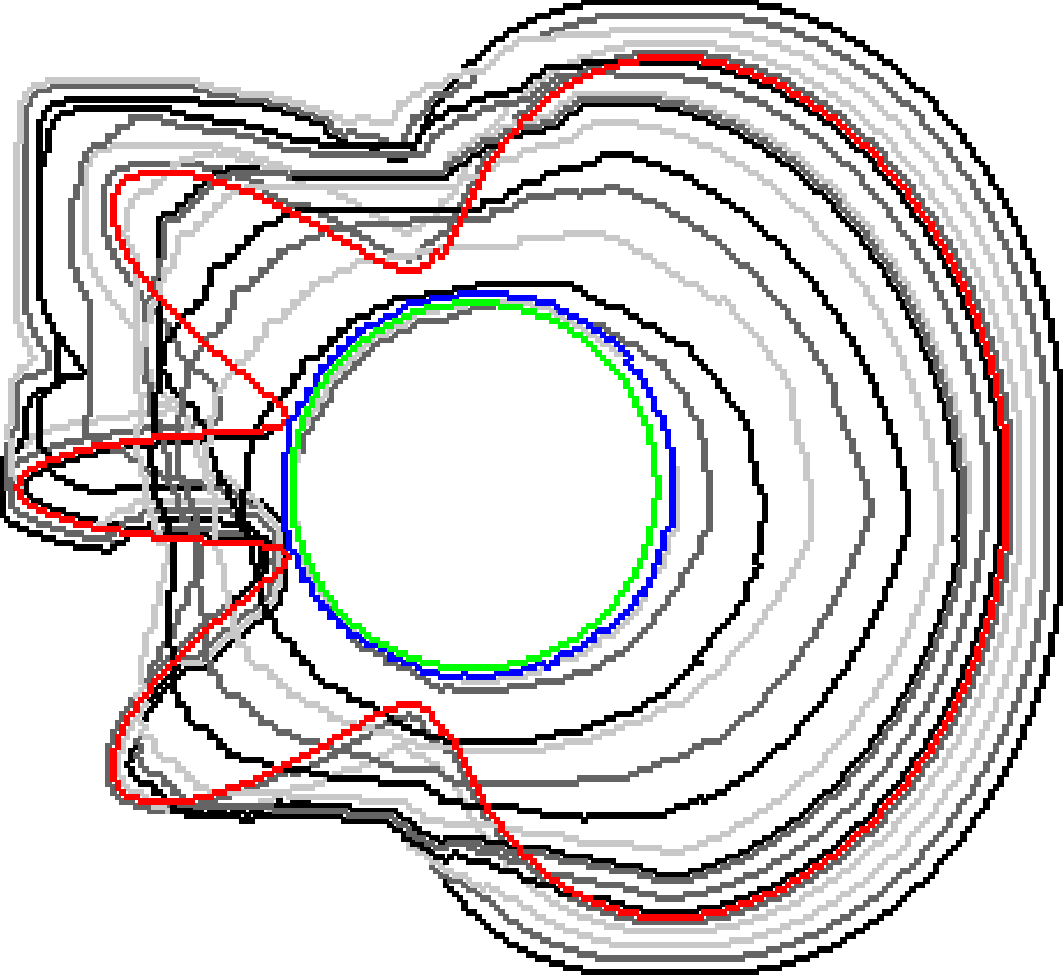
\includegraphics[scale=0.18]{figures/chapter9/free-elastica/localsearch/flower/len_pen-0.01/radius-7/summary.pdf} & 
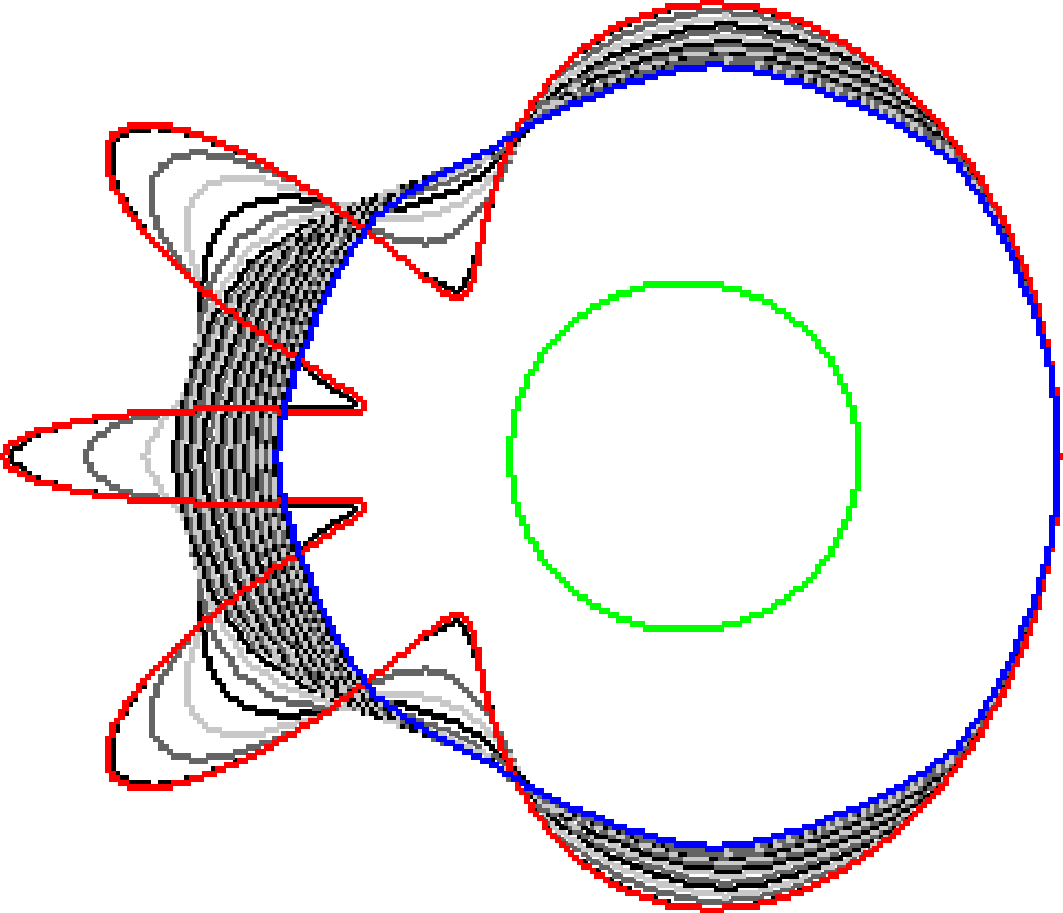
\includegraphics[scale=0.18]{figures/chapter9/free-elastica/flipflow/flower/len_pen-0.01/radius-7/summary.pdf} &
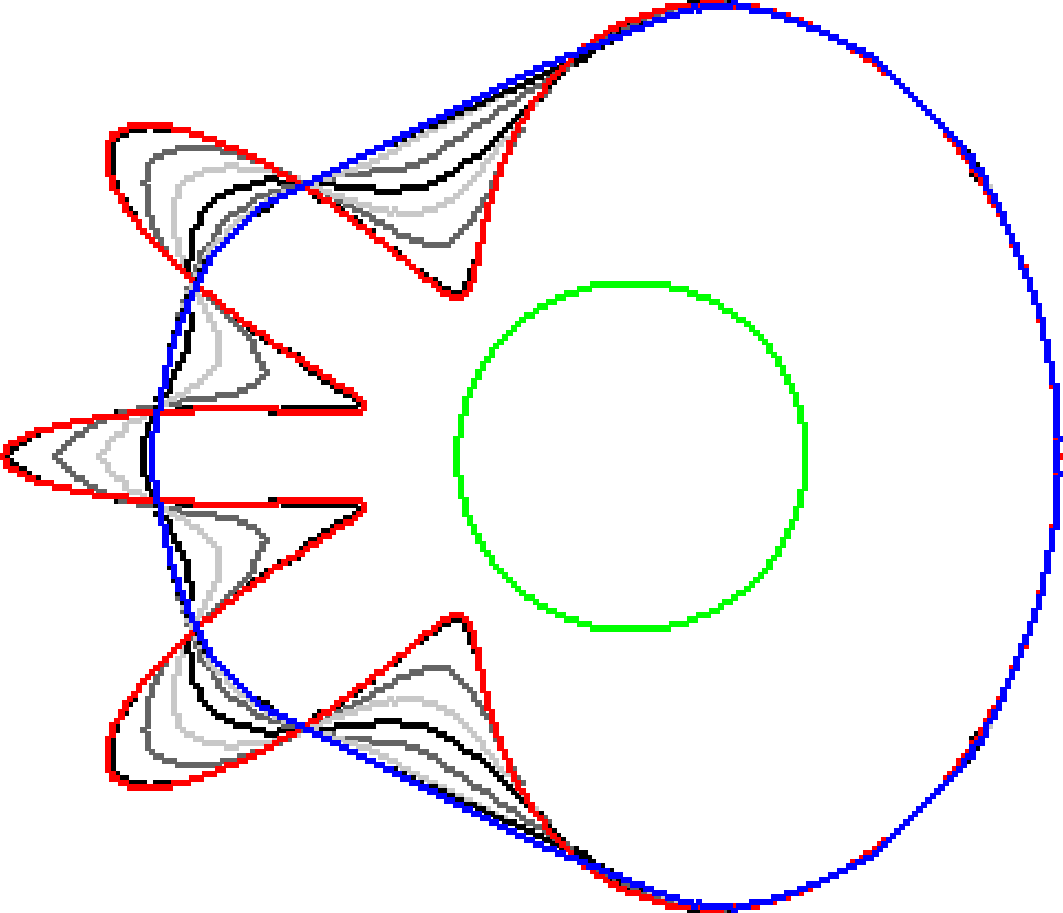
\includegraphics[scale=0.18]{figures/chapter9/free-elastica/balanceflow/flower/len_pen-0.01/radius-7/summary.pdf} &
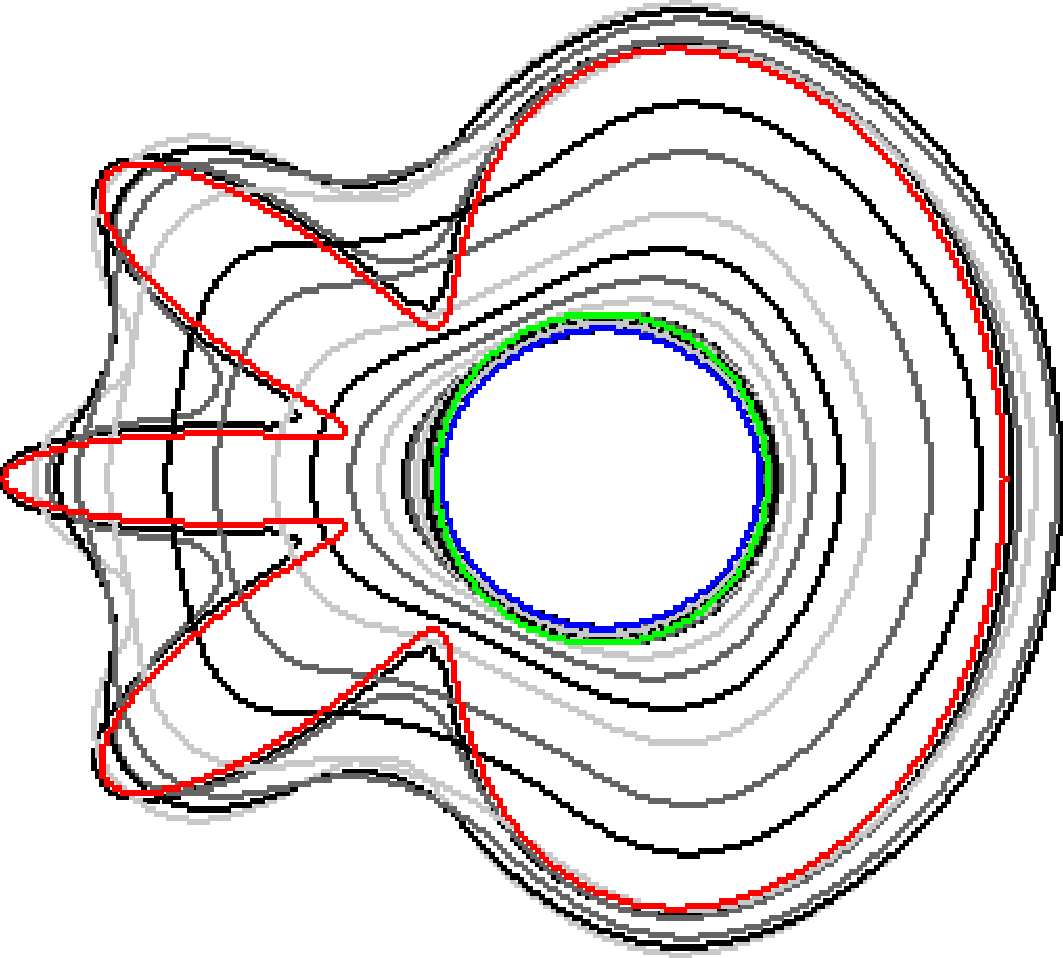
\includegraphics[scale=0.18]{figures/chapter9/free-elastica/graphflow/flower/len_pen-0.01/radius-7/summary.pdf} \\[1em]
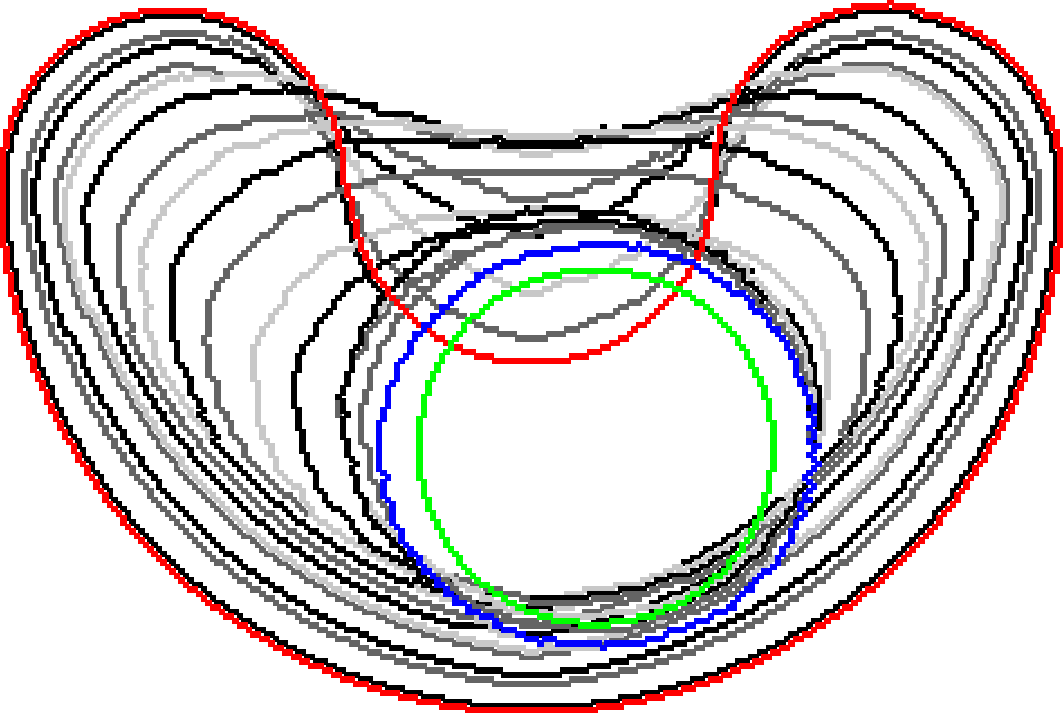
\includegraphics[scale=0.18]{figures/chapter9/free-elastica/localsearch/bean/len_pen-0.01/radius-7/summary.pdf} & 
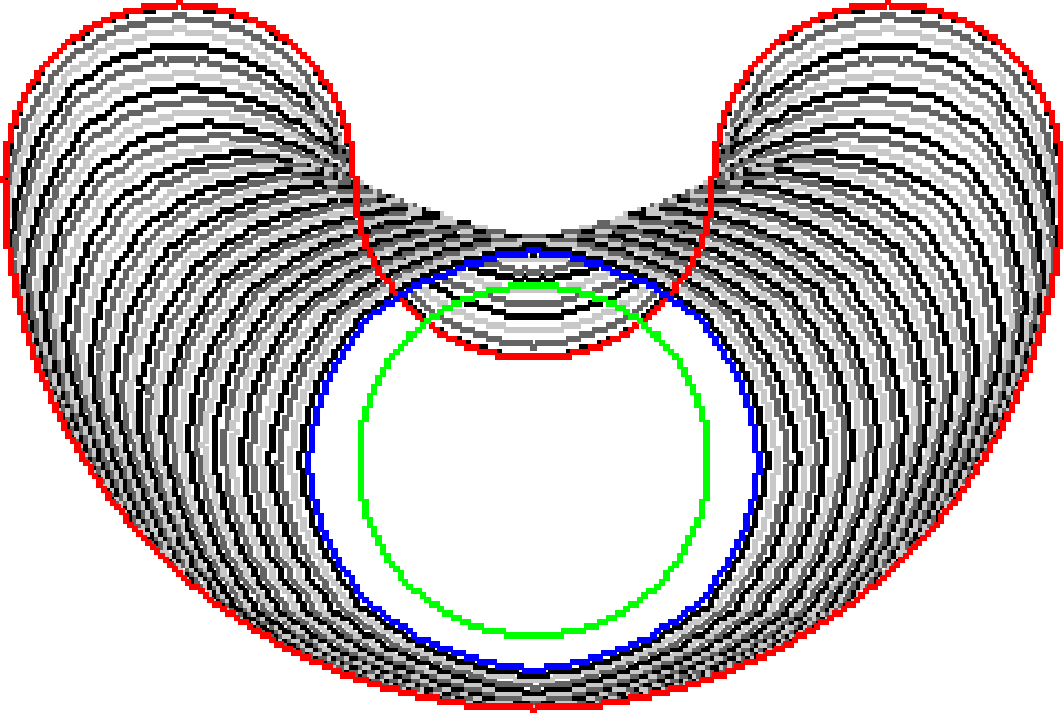
\includegraphics[scale=0.18]{figures/chapter9/free-elastica/flipflow/bean/len_pen-0.01/radius-7/summary.pdf} &
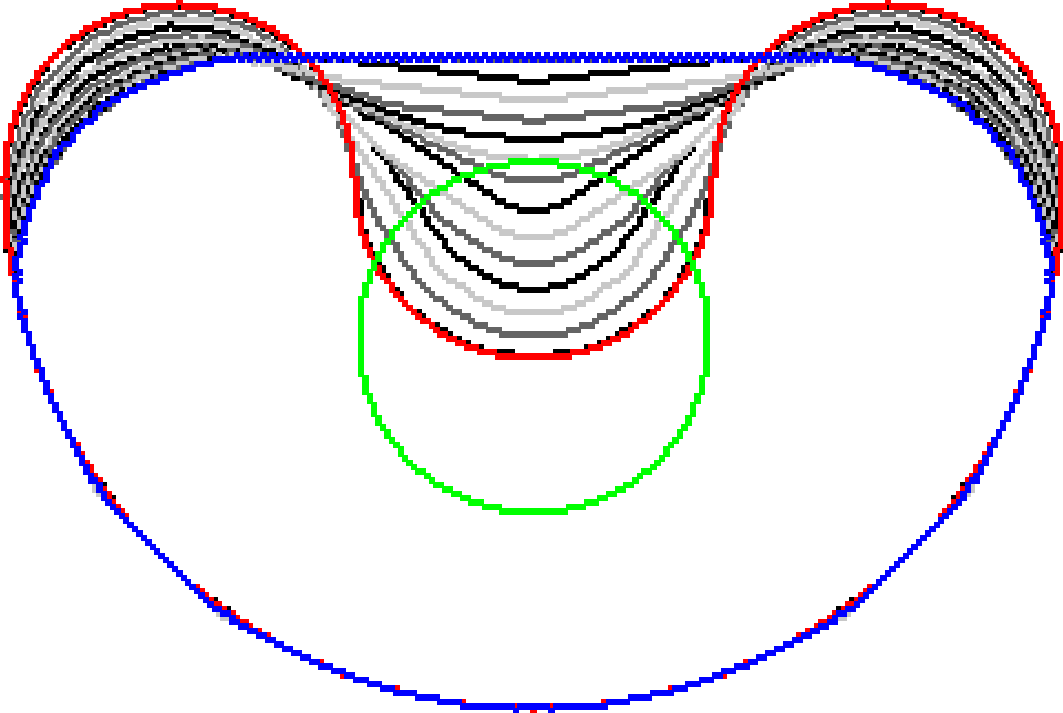
\includegraphics[scale=0.18]{figures/chapter9/free-elastica/balanceflow/bean/len_pen-0.01/radius-7/summary.pdf} &
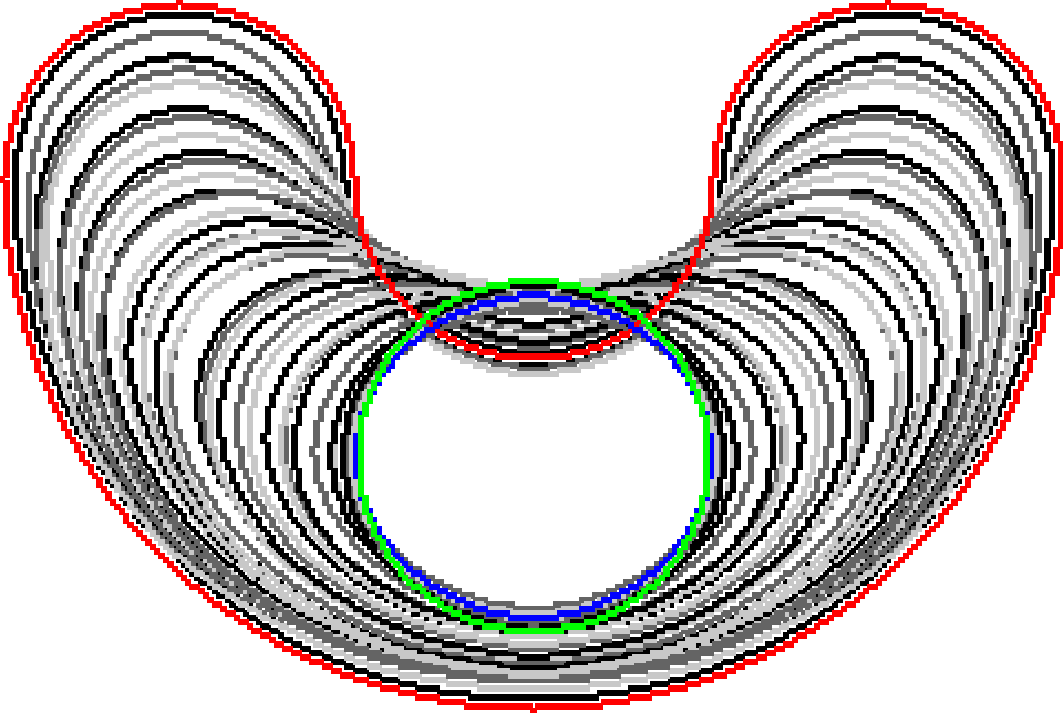
\includegraphics[scale=0.18]{figures/chapter9/free-elastica/graphflow/bean/len_pen-0.01/radius-7/summary.pdf} 
\end{tabular}
\caption{\daniel{\textbf{Exp-General results for the free elastica.}}. Initial contour is colored in red, final contour is colored in blue and optimal contour is colored in green. Curves are drawn every $10$ iterations.}
\label{ch9:fig:results-free-elastica-general}
\end{figure}

\begin{figure}
\begin{tabular}{cc}
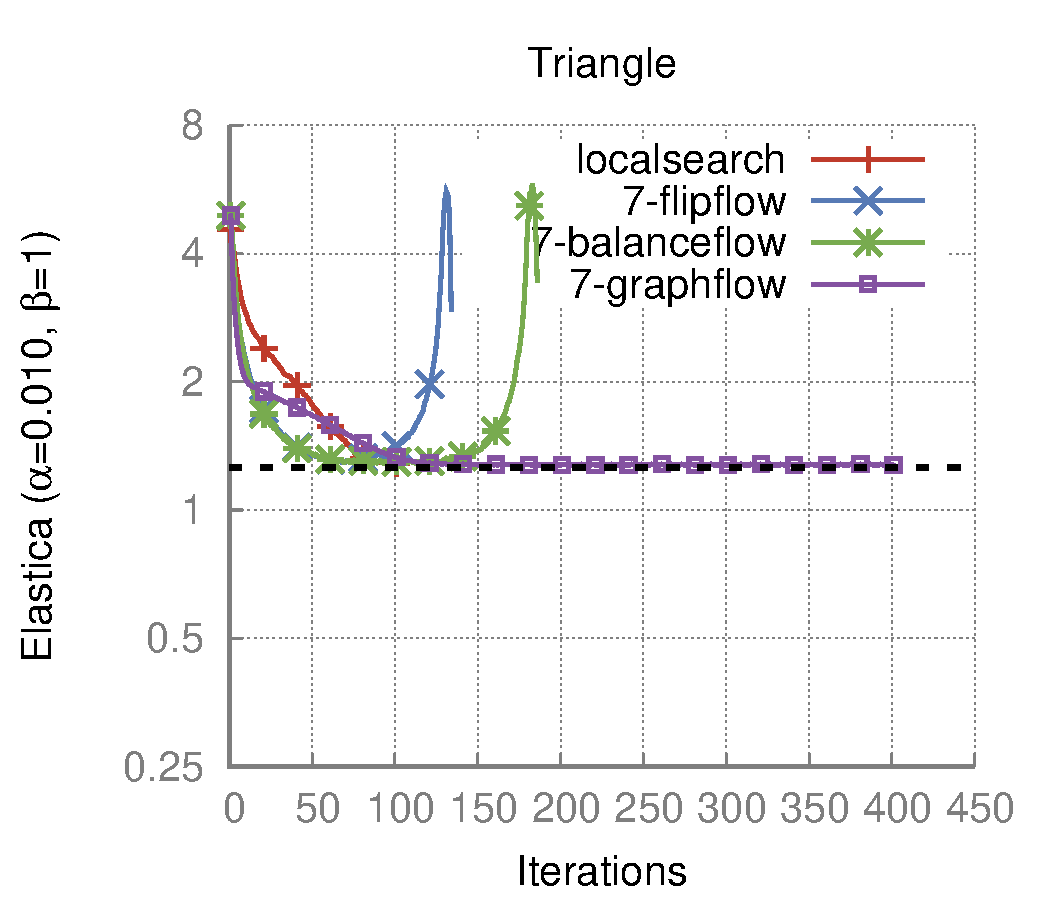
\includegraphics[scale=0.45]{figures/chapter9/free-elastica/plots/iteration/main_experiment/len_pen_0.01/radius-7/triangle.pdf} &
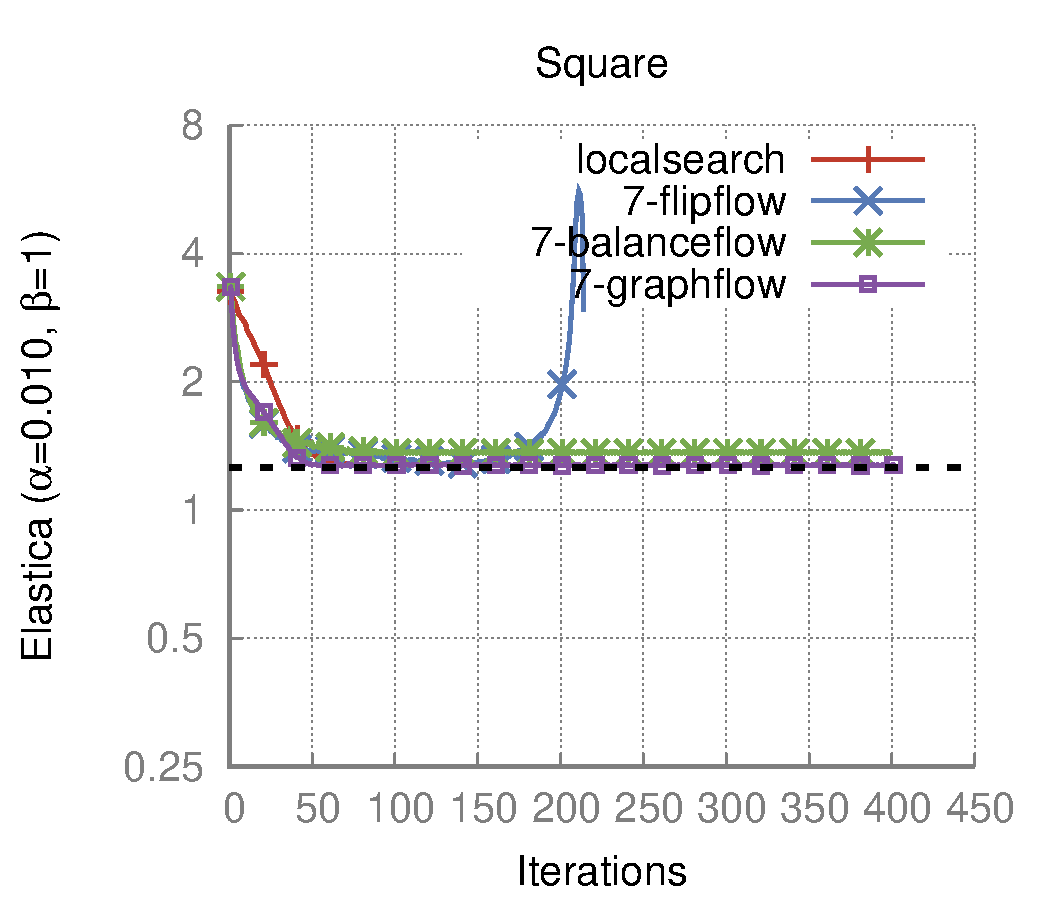
\includegraphics[scale=0.45]{figures/chapter9/free-elastica/plots/iteration/main_experiment/len_pen_0.01/radius-7/square.pdf}\\[1em]
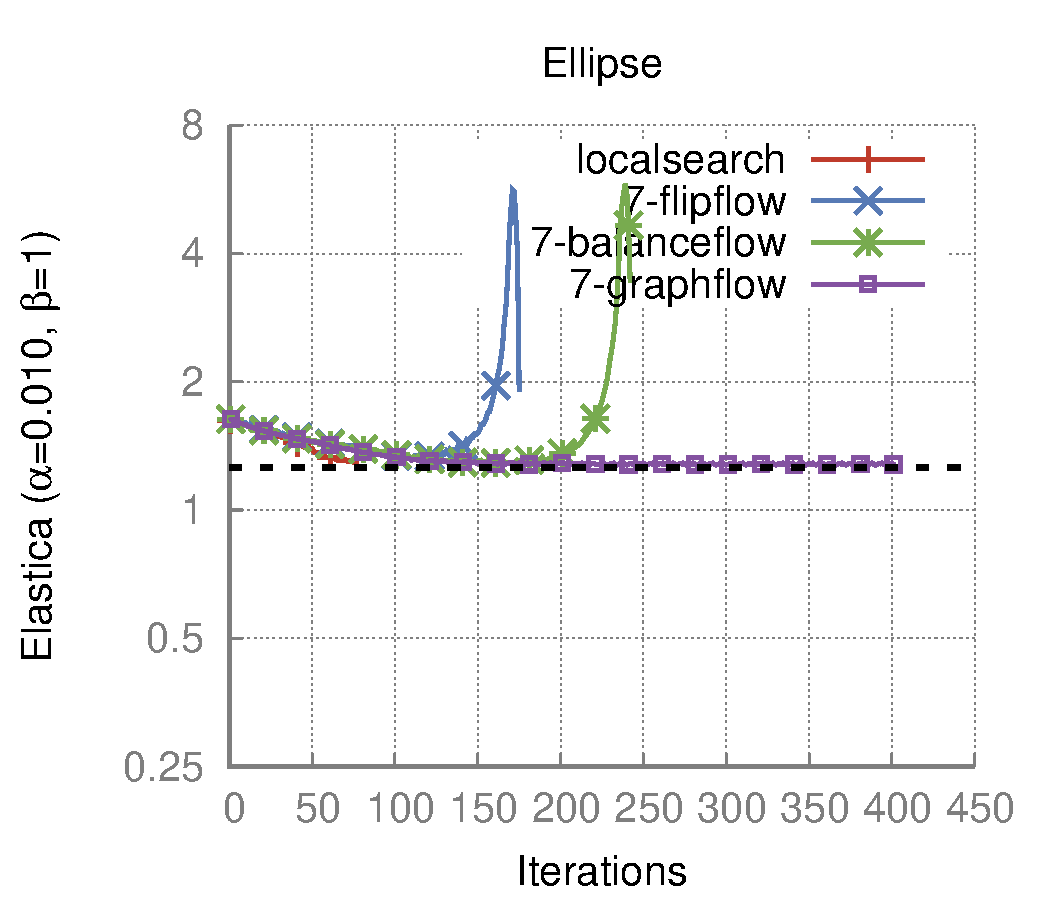
\includegraphics[scale=0.45]{figures/chapter9/free-elastica/plots/iteration/main_experiment/len_pen_0.01/radius-7/ellipse.pdf} &
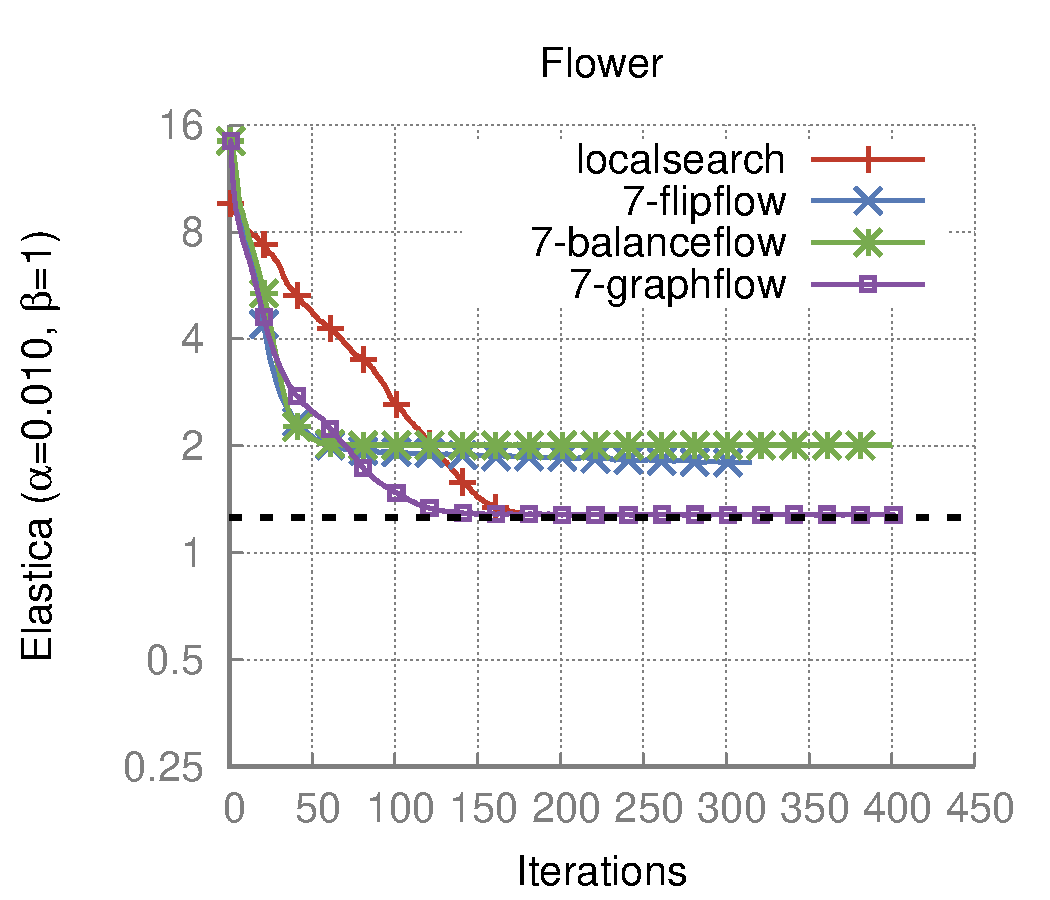
\includegraphics[scale=0.45]{figures/chapter9/free-elastica/plots/iteration/main_experiment/len_pen_0.01/radius-7/flower.pdf}\\[1em]
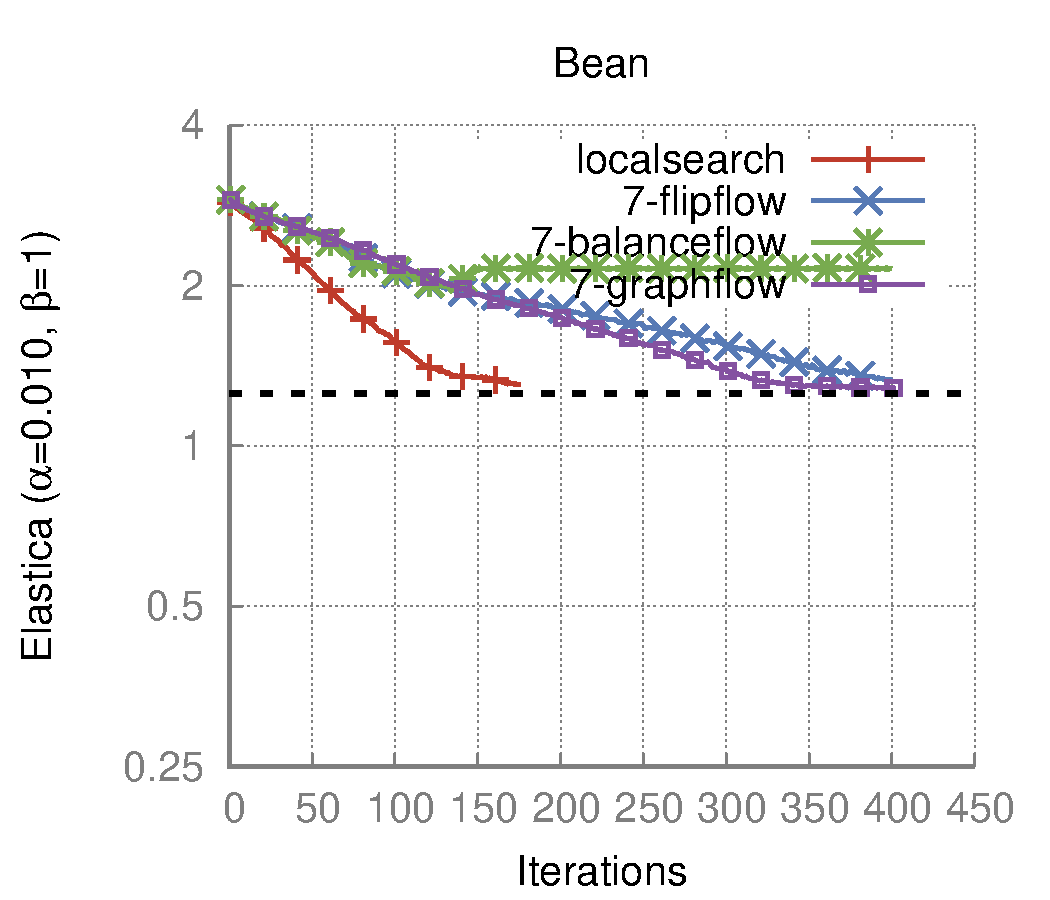
\includegraphics[scale=0.45]{figures/chapter9/free-elastica/plots/iteration/main_experiment/len_pen_0.01/radius-7/bean.pdf}
\end{tabular}
\caption{\daniel{\textbf{Exp-General plots for free elastica}}. LocalSearch and GraphFlow converges to values closer to the global optimum. The dashed line marks the optimum value.}
\label{ch9:fig:plots-free-elastica-general}
\end{figure}

\subsection{Exp-Radius}

In the Exp-Radius experiment, we set the length penalization parameter to $\alpha=0.001$. Compared to the Exp-General, the expected behavior is that the shapes will grow till reach the optimal disk of radius $1/0.001^{0.5} \approx 31$. This experiment confirms the natural observation that the choice of the $bRadius$ parameter influences the produced flows. The experiment was not executed for the LocalSearch model as this model is not sensitive to the $bRadius$ parameter.

In the case of FlipFlow and BalanceFlow, the evolution goes faster with a larger radius, and, as mentioned before, the shape never grows, it only shrinks. On the other hand, GraphFlow is sensitive to the value of $\alpha$ and the shapes can grow or shrink acoordingly. Moreover, the choice of $bRadius$ defines how closer the solution will be from the optimum in the case of the GraphFlow.

\daniel{We recall that the II estimator measures curvature by using a disk of a given radius. The radius parameter defines the range of values estimated by the estimator. At first glance, a larger radius returns a more precise estimation, but we should be careful in not using a radius larger than the reach of the shape at the point of estimation~(see~\cref{ch9:fig:constrained-elastica-underlying-curve-shapes}). A value of $bRadius=7$ is too small to identify the small variations that a shape growing to a disk of radius $31$ suffers. Therefore, when we set $bRadius=12$, the GraphFlow returns solutions closer to the optimal, as we can check in~\cref{ch9:fig:results-free-elastica-radius-choice,ch9:fig:plots-free-elastica-radius-choice}. The results suggests that the $bRadius$ should be dynamically set in order to escape local optimum solutions.}


\begin{figure}
\center
\begin{tabular}{m{1.5cm}ccc}
& FlipFlow & BalanceFlow & GraphFlow\\[1em]
$r=7$ & \raisebox{-.5\height}{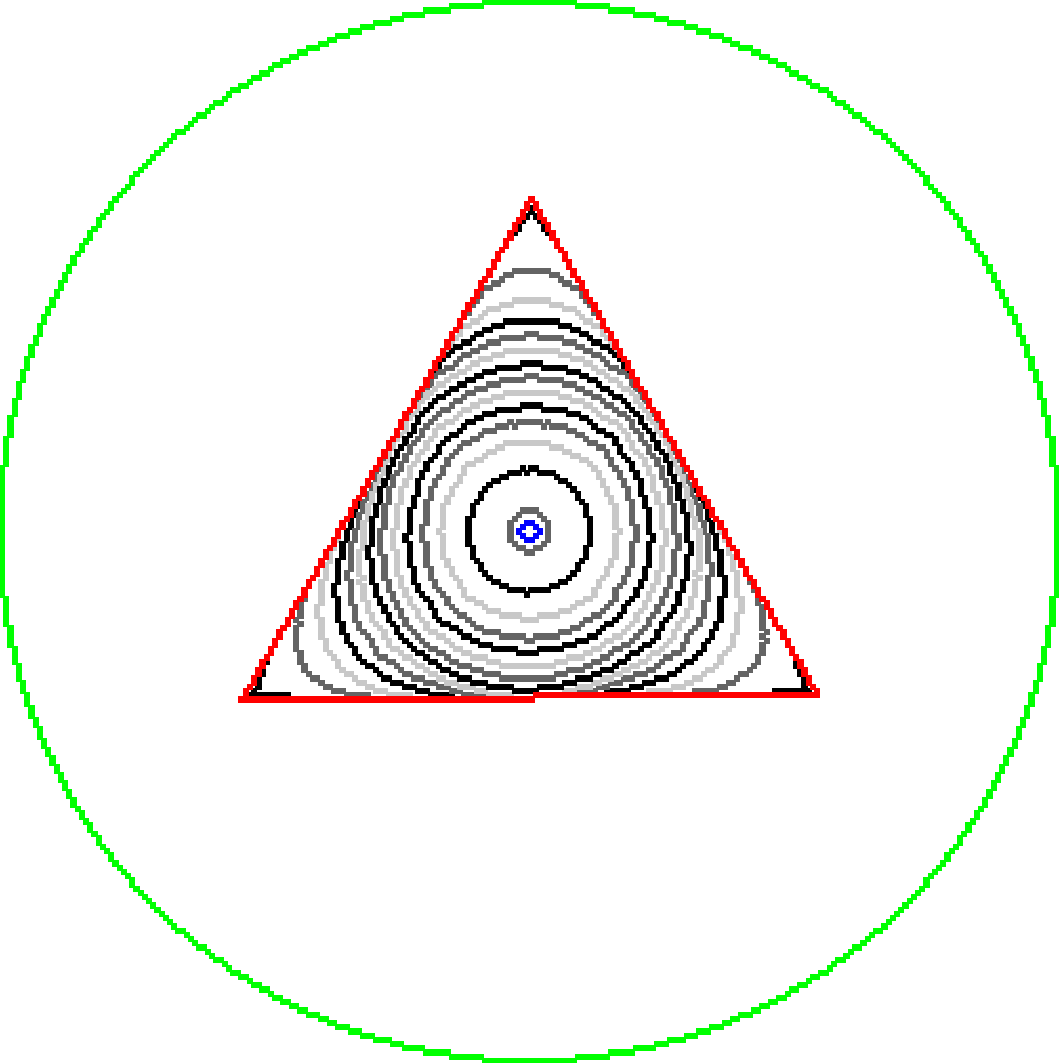
\includegraphics[scale=0.2]{figures/chapter9/free-elastica/flipflow/triangle/len_pen-0.001/radius-7/summary.pdf}} &
\raisebox{-.5\height}{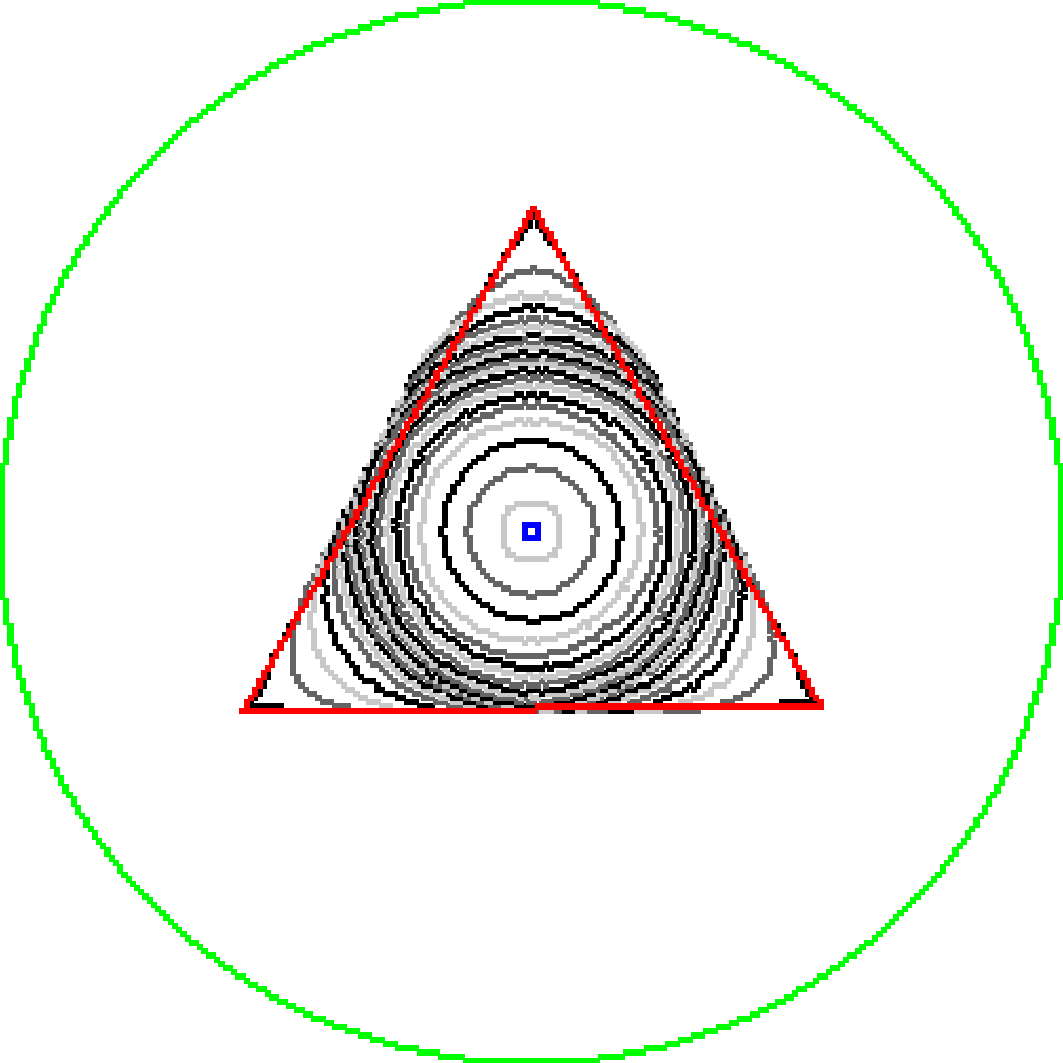
\includegraphics[scale=0.2]{figures/chapter9/free-elastica/balanceflow/triangle/len_pen-0.001/radius-7/summary.pdf}} &
\raisebox{-.5\height}{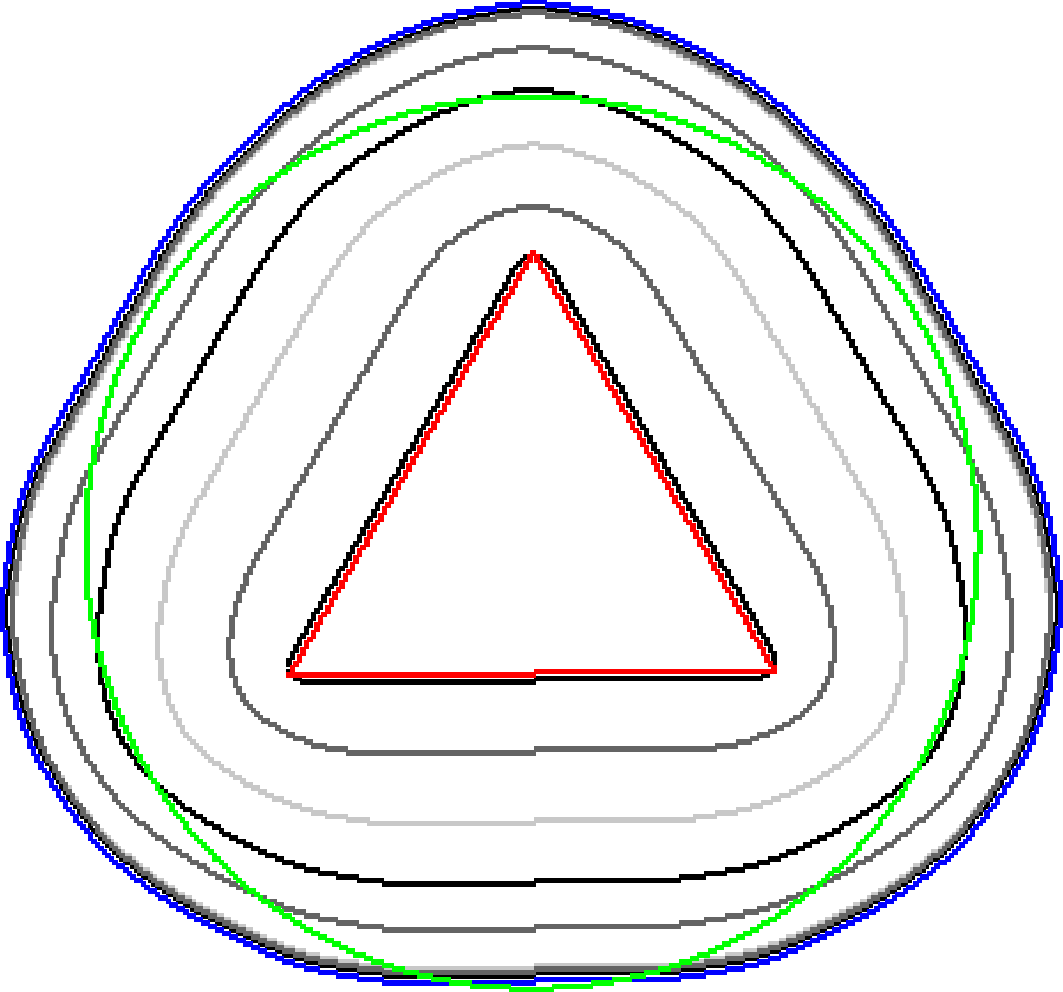
\includegraphics[scale=0.2]{figures/chapter9/free-elastica/graphflow/triangle/len_pen-0.001/radius-7/summary.pdf}} \\[5em]
$r=12$ & \raisebox{-.5\height}{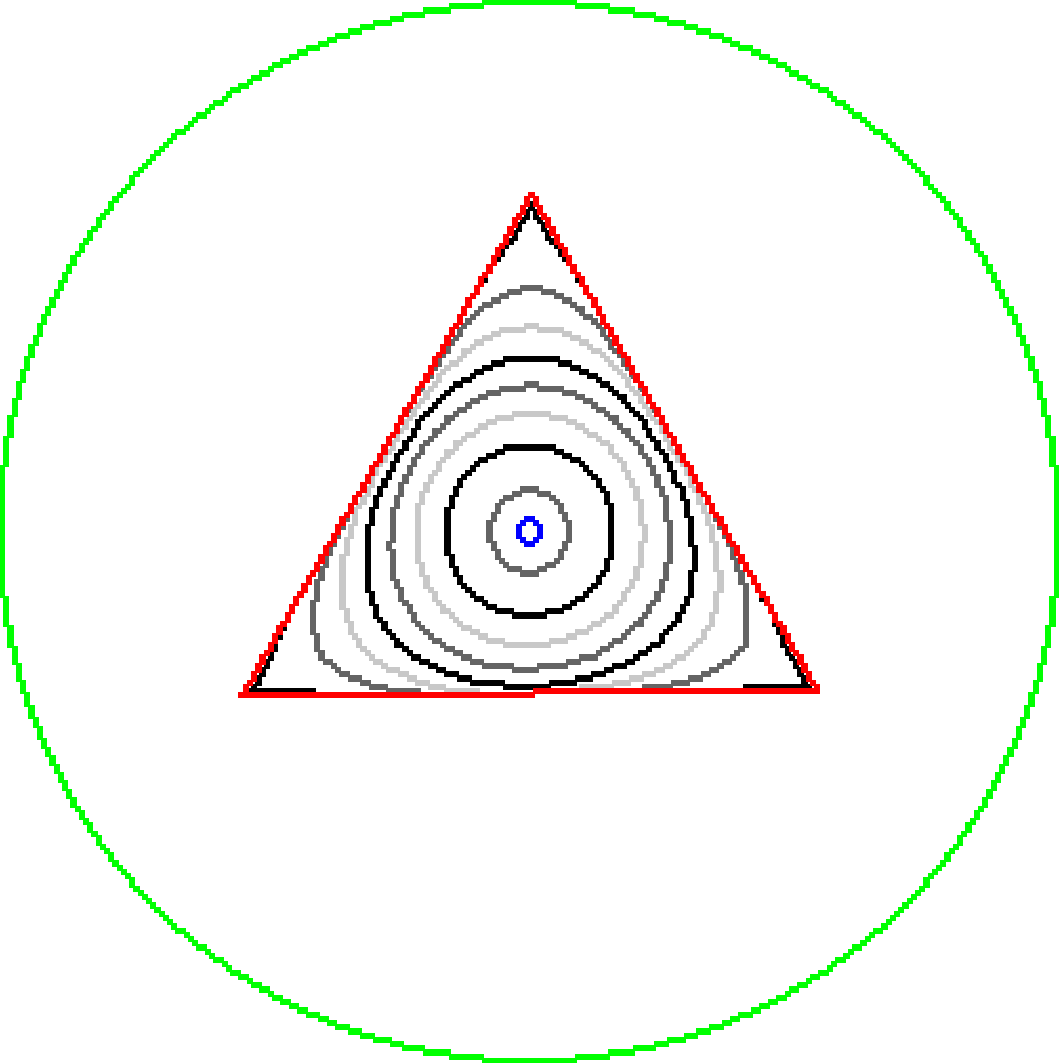
\includegraphics[scale=0.2]{figures/chapter9/free-elastica/flipflow/triangle/len_pen-0.001/radius-12/summary.pdf}} &
\raisebox{-.5\height}{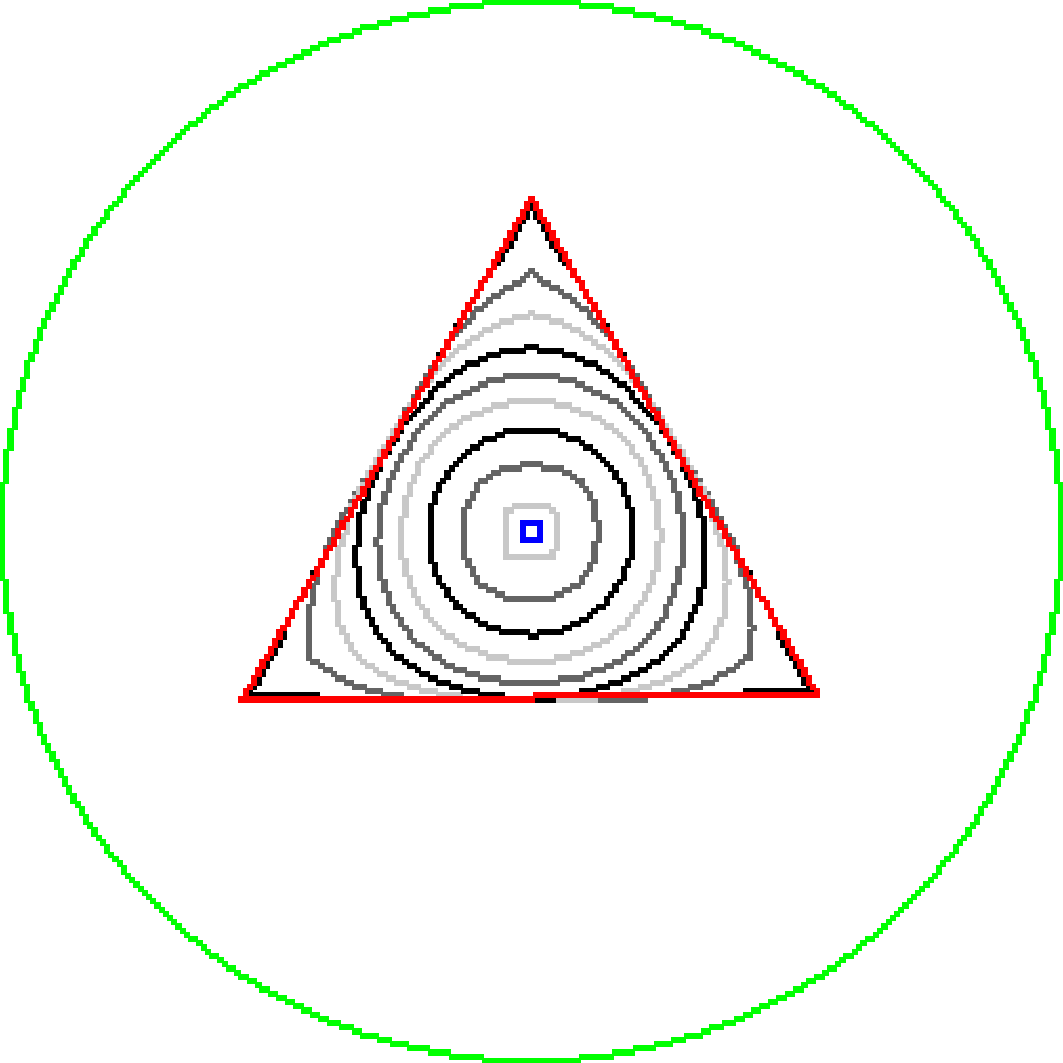
\includegraphics[scale=0.2]{figures/chapter9/free-elastica/balanceflow/triangle/len_pen-0.001/radius-12/summary.pdf}} &
\raisebox{-.5\height}{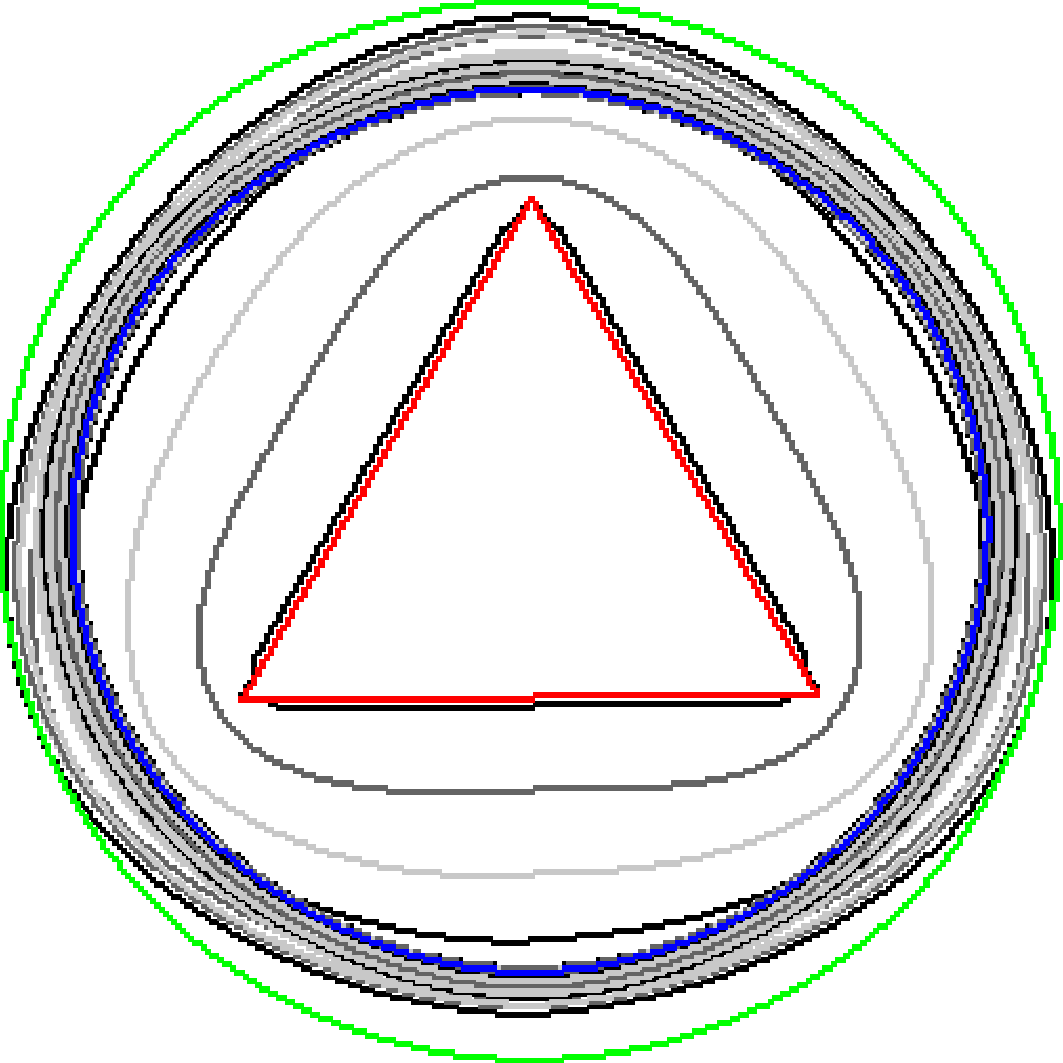
\includegraphics[scale=0.2]{figures/chapter9/free-elastica/graphflow/triangle/len_pen-0.001/radius-12/summary.pdf}} \\[5em]
$r=7$ & \raisebox{-.5\height}{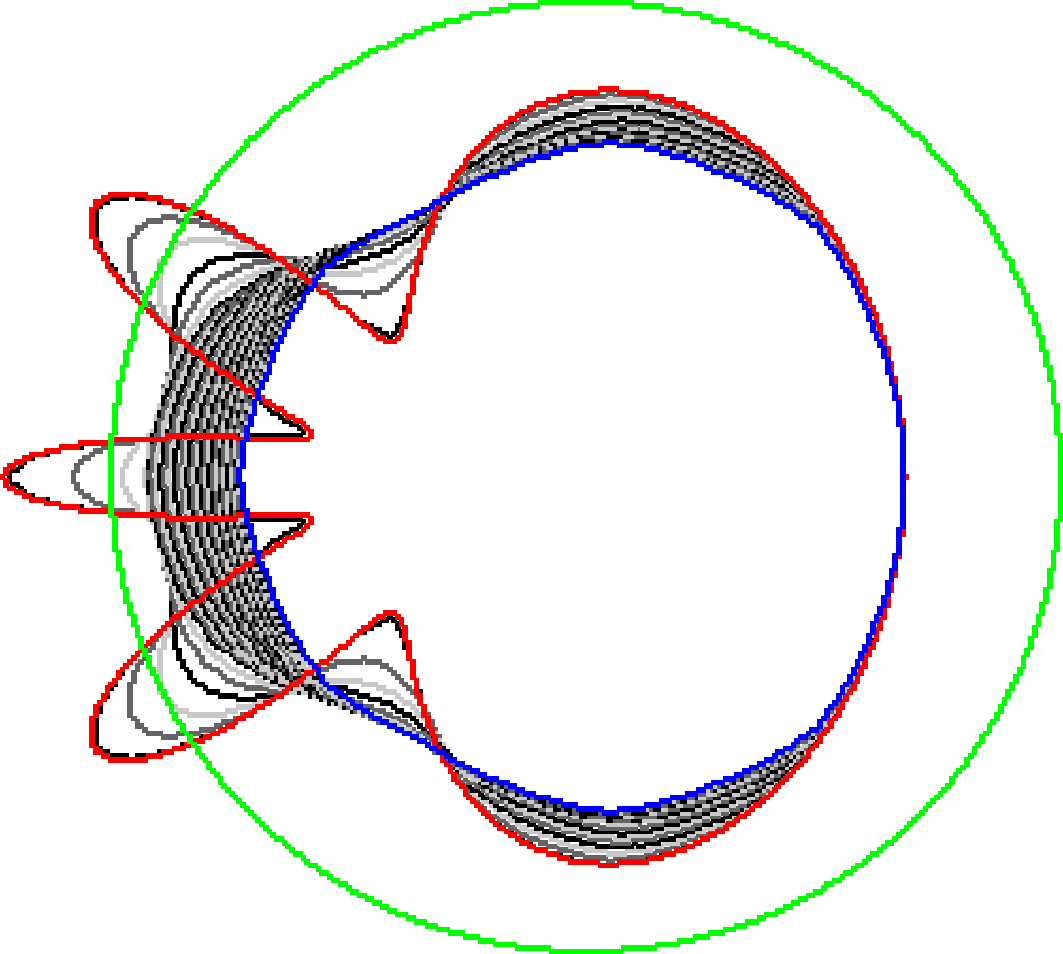
\includegraphics[scale=0.2]{figures/chapter9/free-elastica/flipflow/flower/len_pen-0.001/radius-7/summary.pdf}} &
\raisebox{-.5\height}{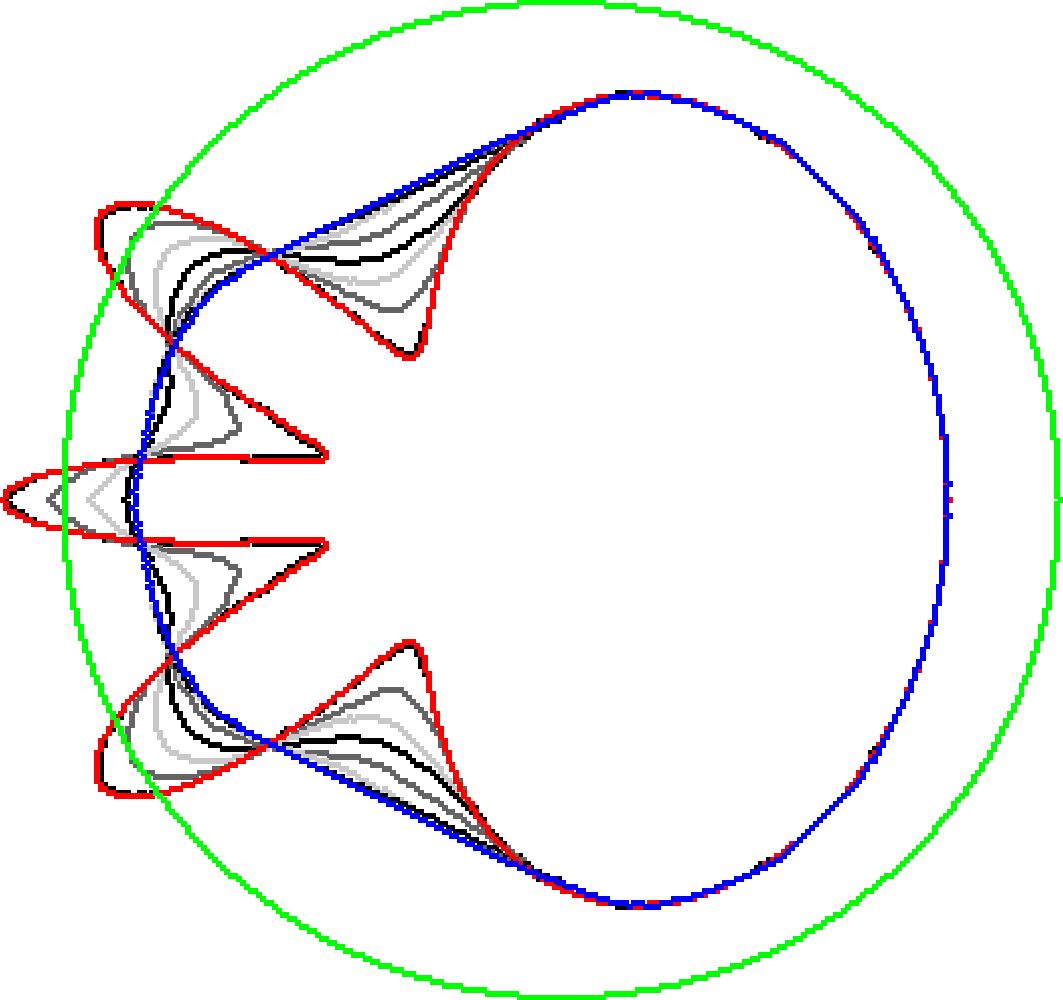
\includegraphics[scale=0.2]{figures/chapter9/free-elastica/balanceflow/flower/len_pen-0.001/radius-7/summary.pdf}} &
\raisebox{-.5\height}{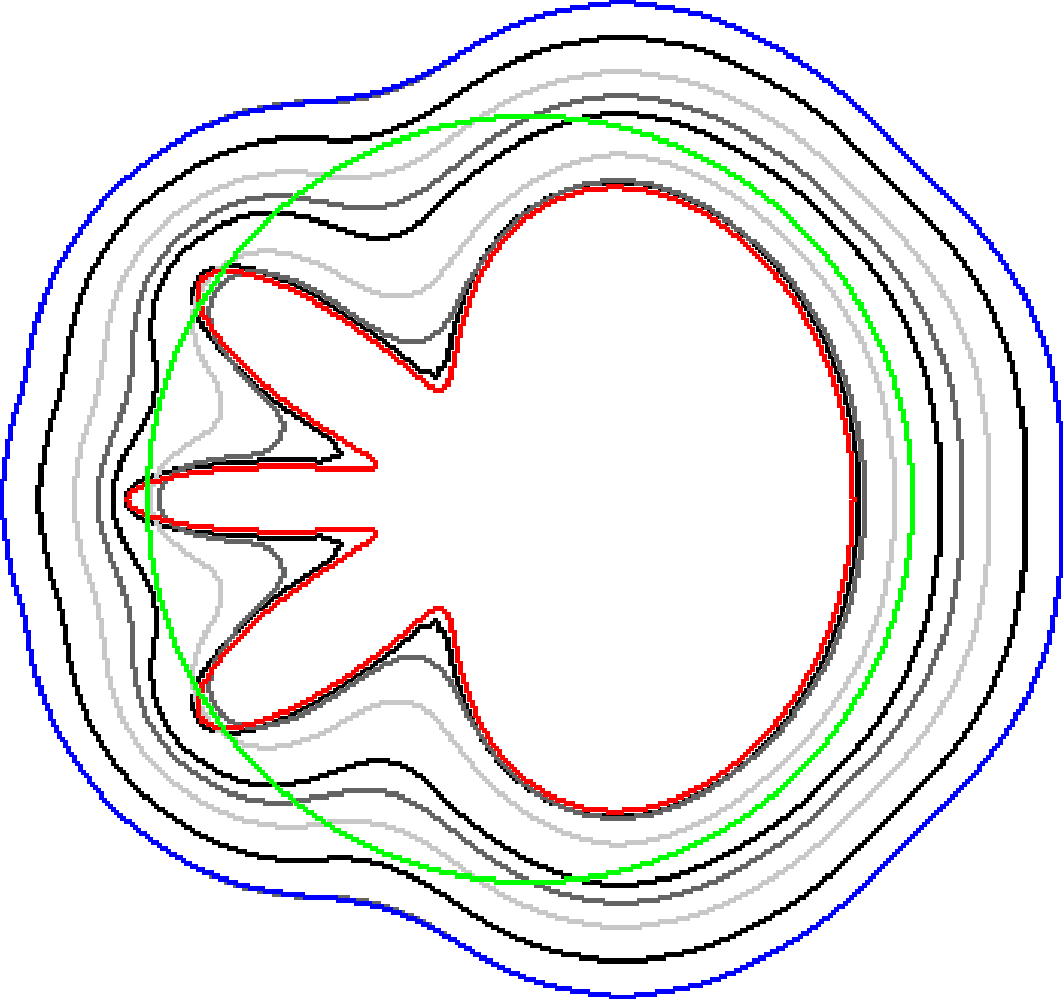
\includegraphics[scale=0.2]{figures/chapter9/free-elastica/graphflow/flower/len_pen-0.001/radius-7/summary.pdf}} \\[5em]
$r=12$ & \raisebox{-.5\height}{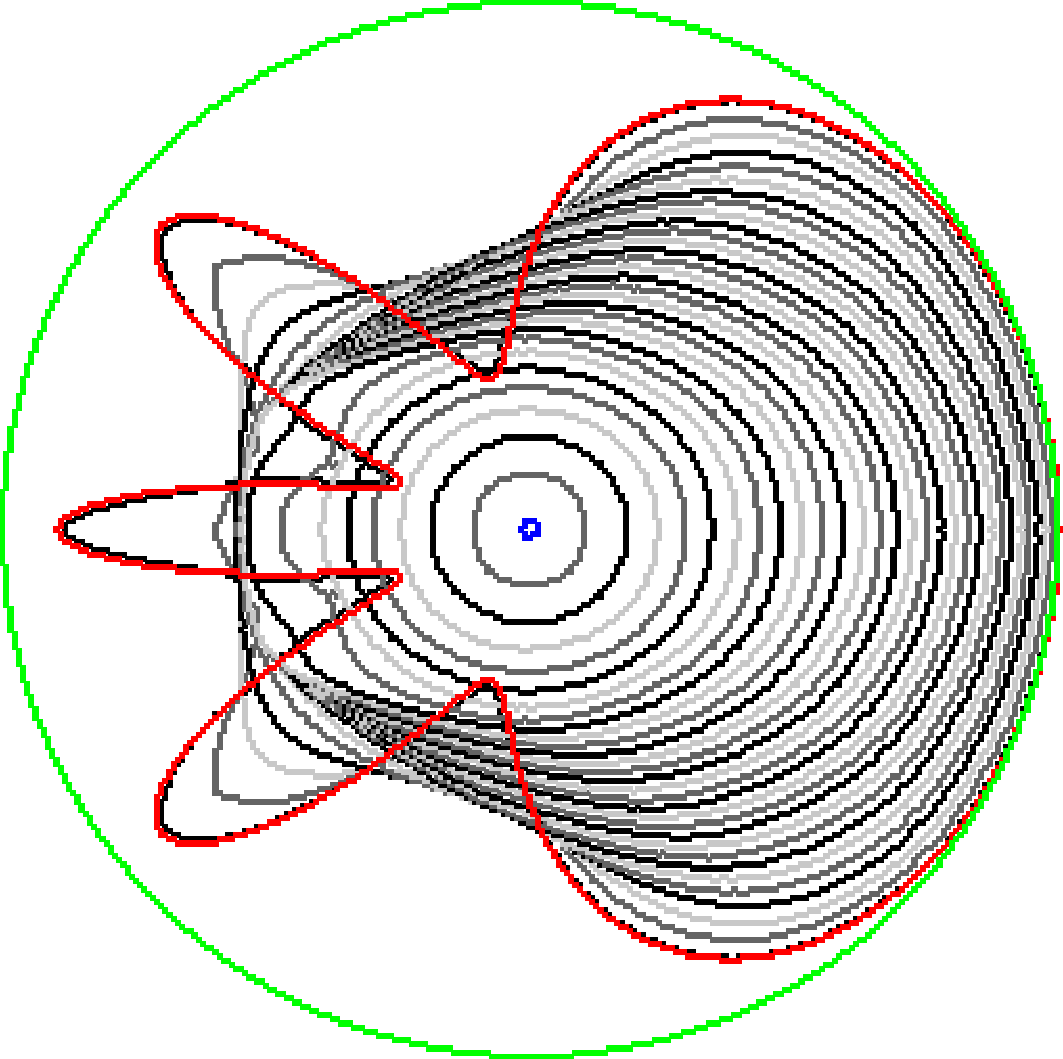
\includegraphics[scale=0.2]{figures/chapter9/free-elastica/flipflow/flower/len_pen-0.001/radius-12/summary.pdf}} &
\raisebox{-.5\height}{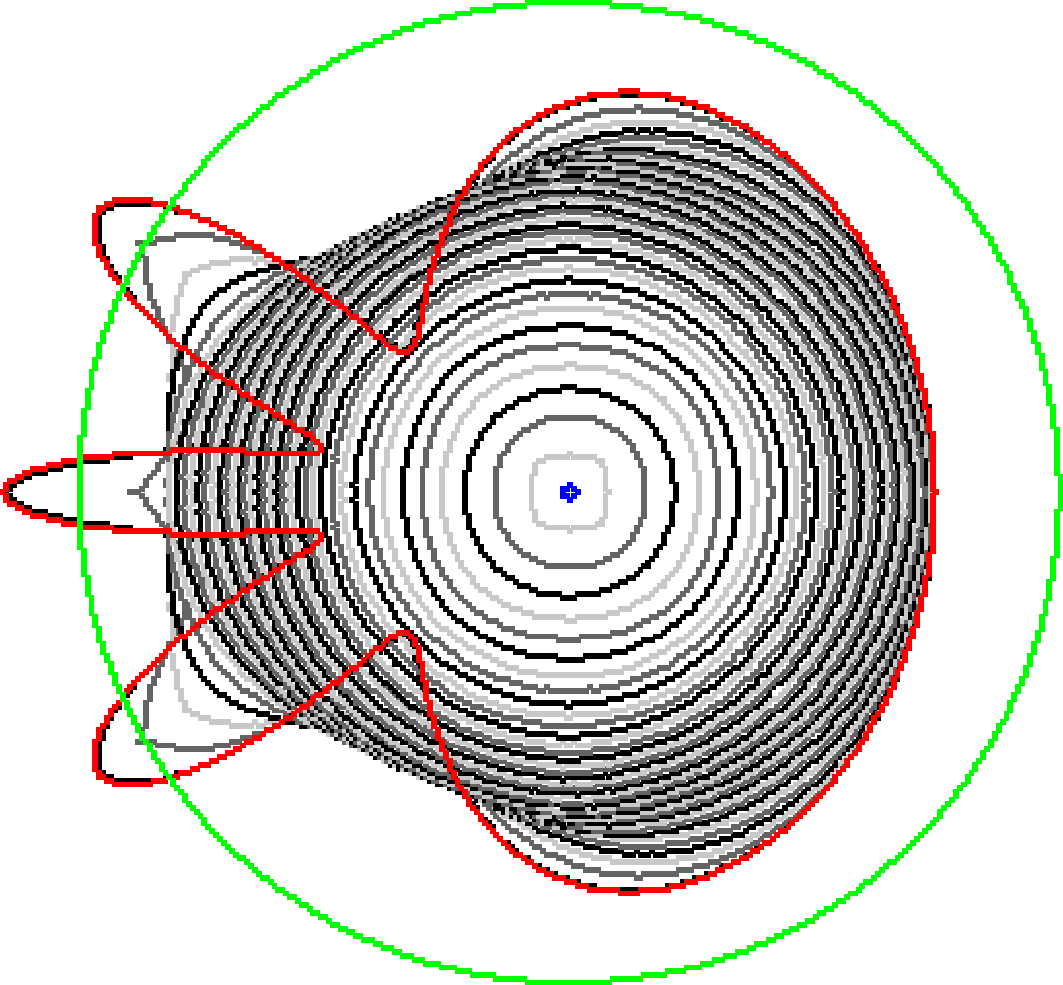
\includegraphics[scale=0.2]{figures/chapter9/free-elastica/balanceflow/flower/len_pen-0.001/radius-12/summary.pdf}} &
\raisebox{-.5\height}{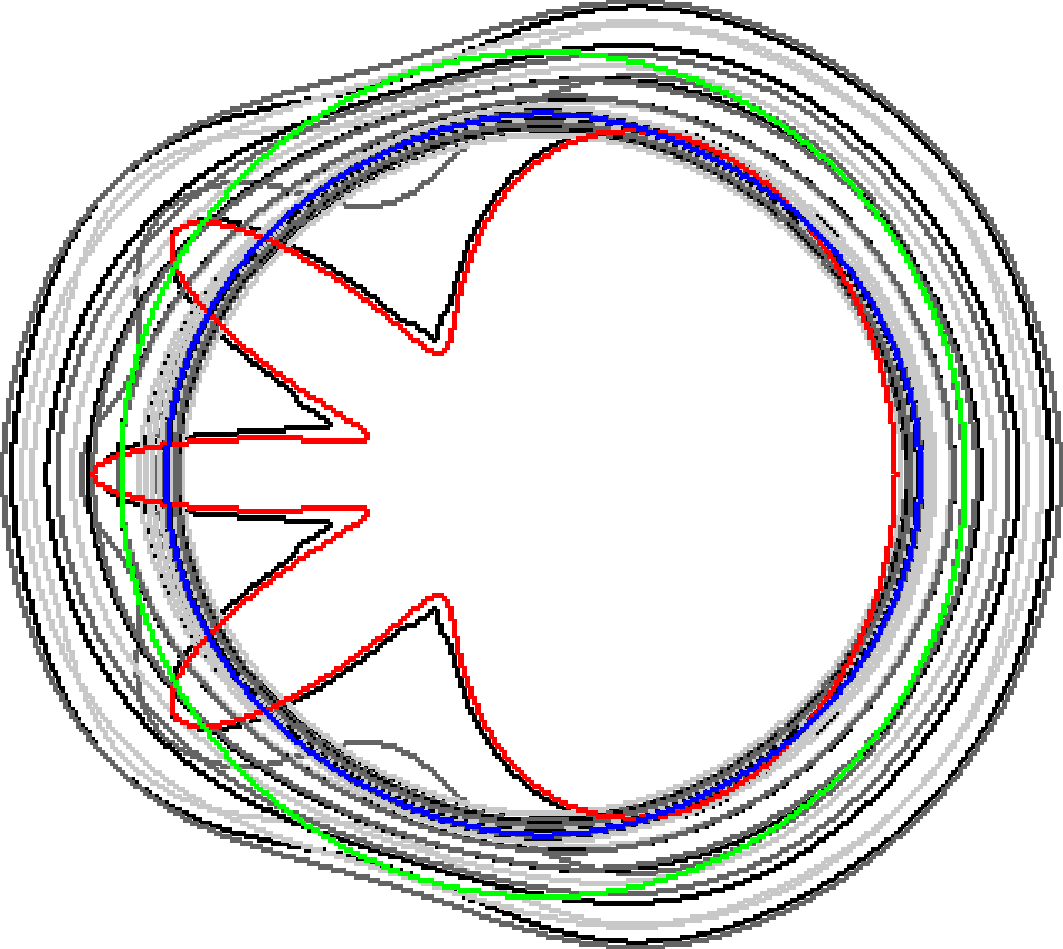
\includegraphics[scale=0.2]{figures/chapter9/free-elastica/graphflow/flower/len_pen-0.001/radius-12/summary.pdf}}
\end{tabular}
\caption{\daniel{\textbf{Exp-Radius results for the free elastica.} A small value of $bRadius$ may not be sufficient to identify small variations in smooth shapes, resulting in a premature on a local minimum. We clearly observe this behavior in the GraphFlow model.} Initial contour is colored in red, final contour is colored in blue and optimal contour is colored in green. Curves are drawn every $10$ iterations.}
\label{ch9:fig:results-free-elastica-radius-choice}
\end{figure}

\begin{figure}
\begin{tabular}{cc}
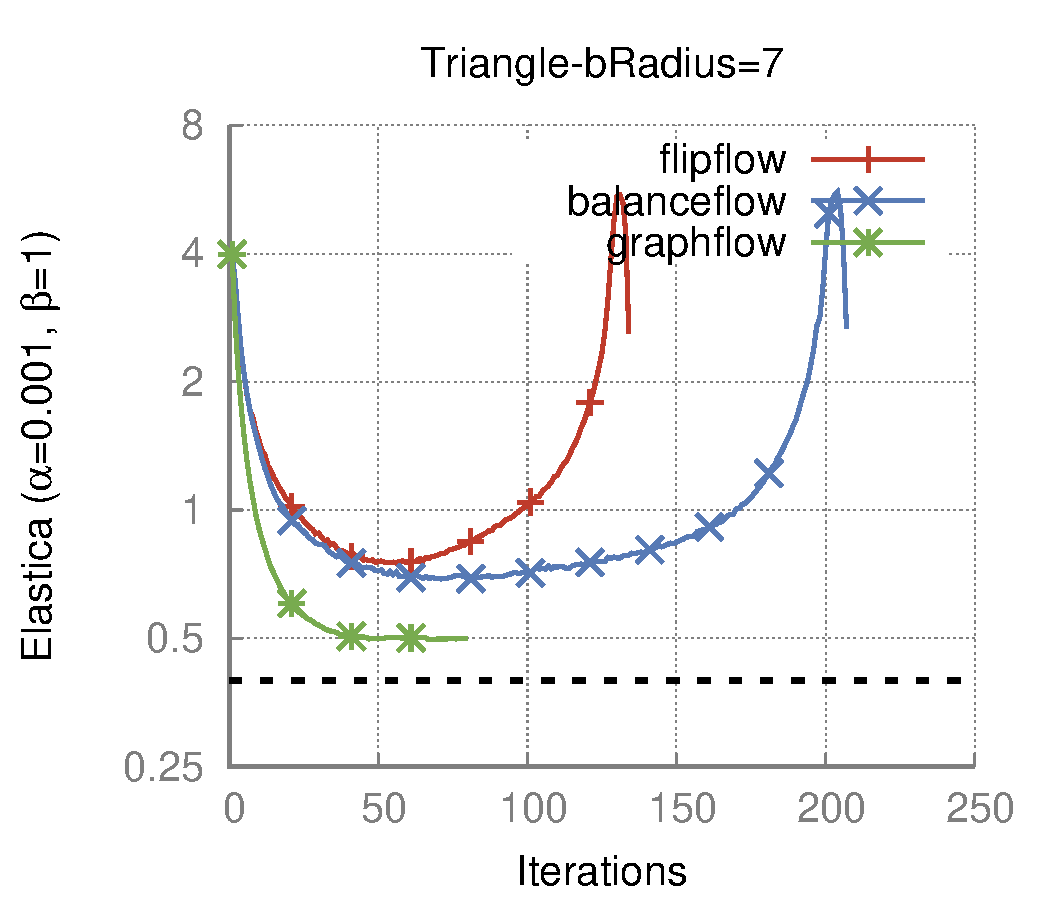
\includegraphics[scale=0.4]{figures/chapter9/free-elastica/plots/iteration/radius_choice/len_pen_0.001/radius-7/triangle.pdf} & 
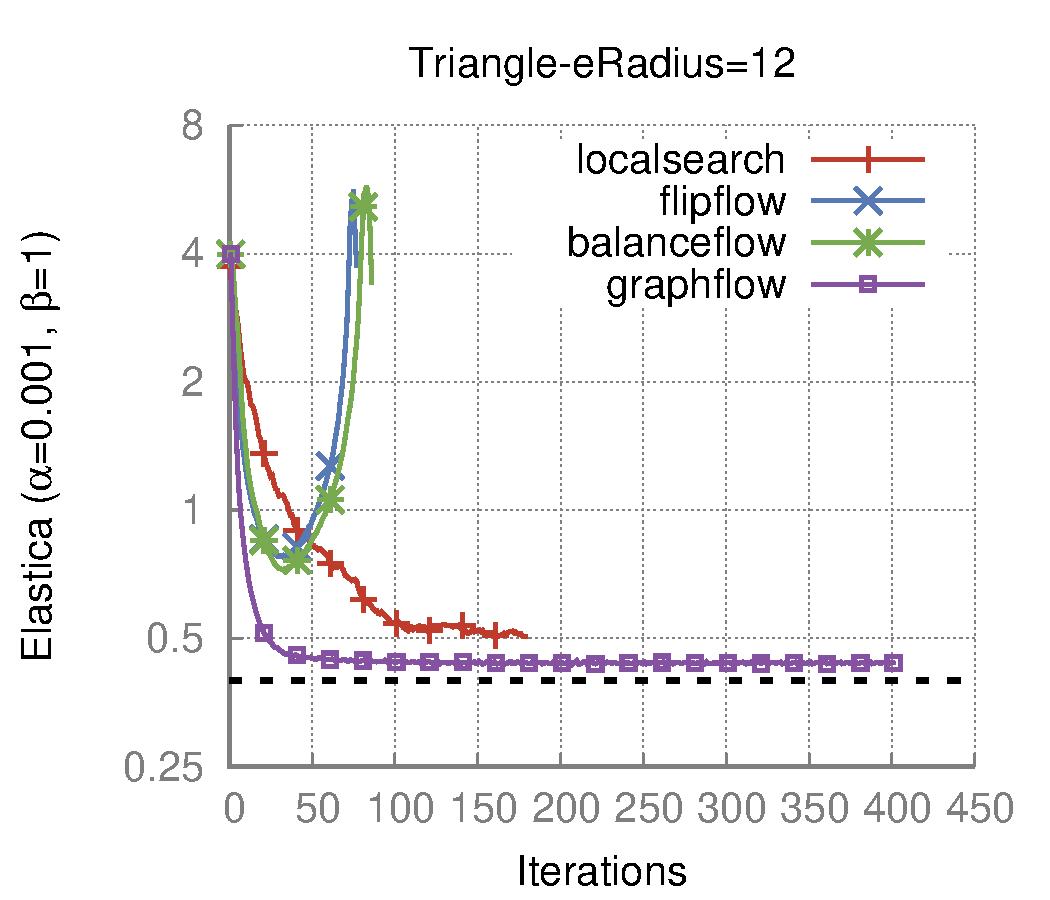
\includegraphics[scale=0.4]{figures/chapter9/free-elastica/plots/iteration/radius_choice/len_pen_0.001/radius-12/triangle.pdf}\\[1em] 
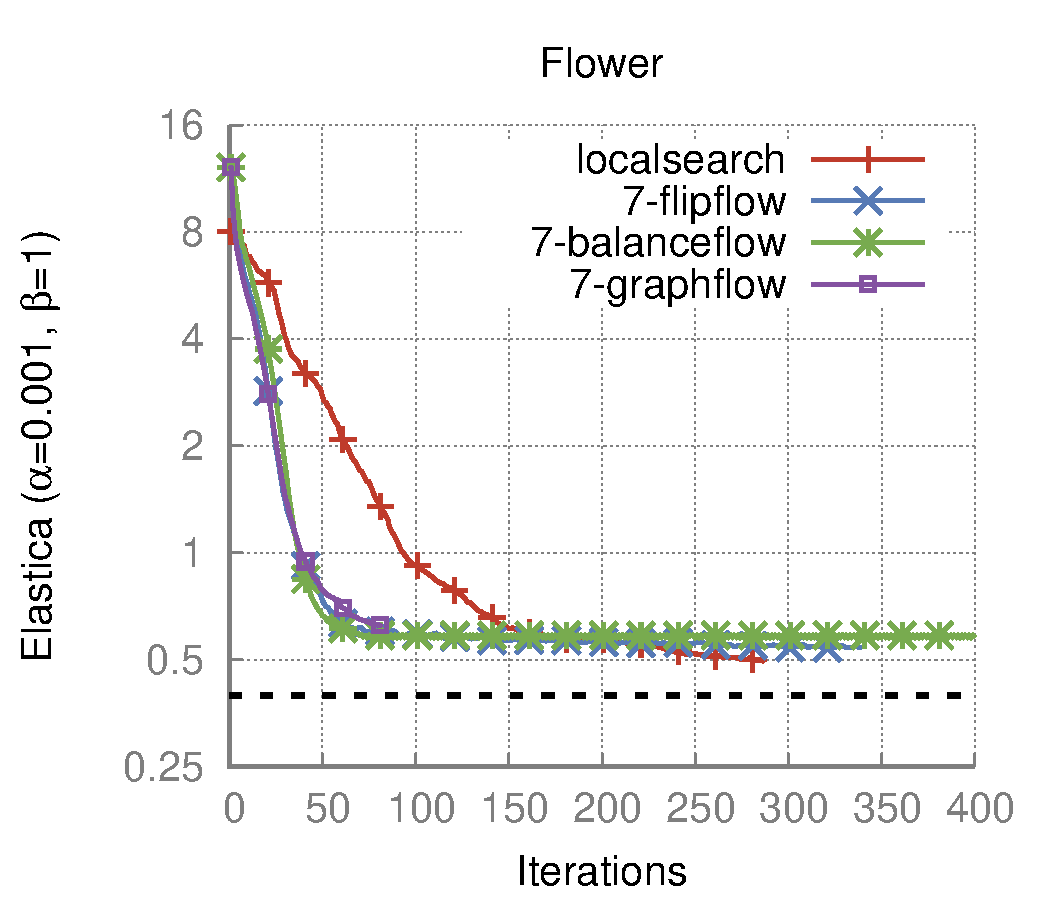
\includegraphics[scale=0.4]{figures/chapter9/free-elastica/plots/iteration/radius_choice/len_pen_0.001/radius-7/flower.pdf} & 
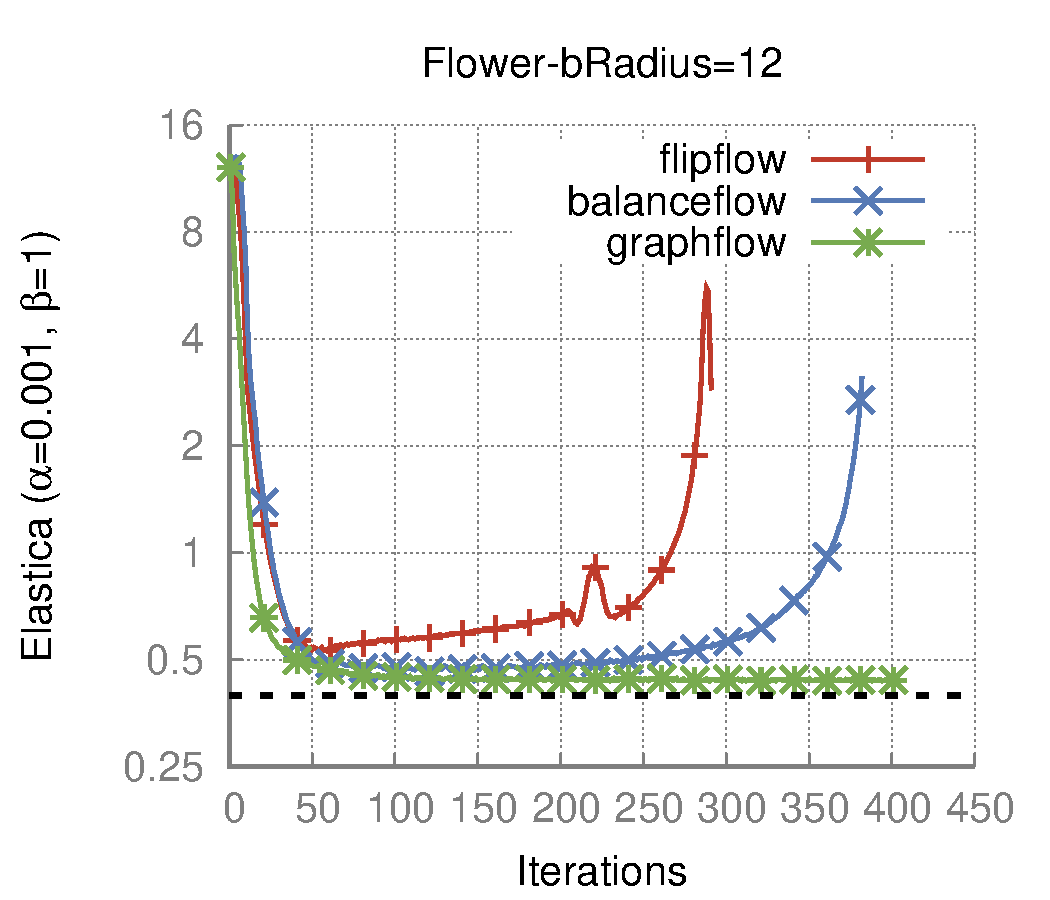
\includegraphics[scale=0.4]{figures/chapter9/free-elastica/plots/iteration/radius_choice/len_pen_0.001/radius-12/flower.pdf}
\end{tabular}
\caption{\daniel{\textbf{Exp-Radius plots for the free elastica.} The GraphFlow approaches values closer to the global optimum when choosing a higher value for $bRadius$ in the case $\alpha =0.001$.}}
\label{ch9:fig:plots-free-elastica-radius-choice}
\end{figure}


\section{Constrained elastica}

The constrained elastica problem consists in finding the shape of minimum digital elastica that respects some set of constraints. We ran experiments for two sets of constraints: in the first, we impose that a set of pixels in the digital boundary of the initial shape must persist in the final shape; in the second, we evolve a curve whose endpoints' orientations are fixed. 

For the constrained elastica, only LocalSearch and GraphFlow were evaluated. We believe that both FlipFlow and BalanceFlow can be modified to evolve the constrained elastica, but such modifications were not implemented in this thesis.~\cref{ch9:tab:constrained-elastica-parameters-summary} lists the parameters used in the experiments and~\cref{ch9:tab:rtime-constrained-elastica-general} the running time of Exp-$\alpha$ experiment.

\begin{table}
\centering
\begin{tabular}{|c|c|c|c|c|c|c|c|c|}
\cline{8-9}
\multicolumn{7}{c|}{} & \multicolumn{2}{|c|}{GF}\\
\hline
Experiment & $maxIt$ & $vRadius$ & $bRadius$ & $h$ & $\alpha$ & $\beta$ & $a$ & $n$ \\
\hline
\multirow{2}{*}{Exp-$\alpha$} & \multirow{2}{*}{$400$} & \multirow{2}{*}{$7$} & \multirow{2}{*}{$7$} & \multirow{2}{*}{$1.0$} & $0.002$ & \multirow{2}{*}{$1$} & \multirow{2}{*}{$1$} & \multirow{2}{*}{$2$} \\
& & & & & $0.0002$ & & &\\
\hline
\multirow{2}{*}{Exp-Radius} & \multirow{2}{*}{$400$} & $15$ & $15$ & \multirow{2}{*}{$1.0$} & \multirow{2}{*}{$0.002$} & \multirow{2}{*}{$1$} & \multirow{2}{*}{$1$} & \multirow{2}{*}{$2$} \\
& & $50$ & $50$ & & & & &\\
\hline
\end{tabular}
\caption{\daniel{\textbf{Parameter settings for the constrained elastica experiments}}. The headers LS,GF identifies parameters that are exclusive for the LocalSearch and GraphFlow models, respectively.}
\label{ch9:tab:constrained-elastica-parameters-summary}
\end{table}

We remark that for every experiment in this section the grid step is set to $h=1.0$, i.e., the Euclidean and digital radius are the same. In contrast with the previous section, where all the shapes had a closed parametric formula, some of the tested shapes in this section are created ad-hoc and a decision about the grid step in this case becomes arbitrary.
\daniel{
\subsubsection{Note about implementation}
In the LocalSearch model, we simply ignore the solutions which do not respect the constraints. In the GraphFlow model, we judiciously set the cost function to guarantee that pixels marked fixed will belong to the source component of the cut and will remain a pixel of the digital contour. 

Let $A \subset D$ be the set of fixed pixels of digital set $D$ and $A' \not\subset D$ their neighbors not contained in $D$. Next, we set the following edge capacities 
\begin{align*}
c( ( s,v_a ) ) &= M, \quad \forall a \in A \\
c( ( v_{a'},t ) ) &= M, \quad \forall a' \in A',
\end{align*}
where $M$ is set as the highest capacity of the graph.
\subsection{Discussion}
The results show that the GF model is not appropriate to solve the constrained elastica problem and we identify two reasons for that. 
\begin{itemize}
\item[]{\textbf{Poor shape neighborhood}. The $a$-probe set promotes quite rough and simple transformations to capture the fine information around the fixed pixels, and we confirm this hypothesis by comparing the GF results with those of the LS model, much more suitable for this kind of task because of its heterogeneous neighborhood.}
\item[]{\textbf{Unresponsiveness of balance coefficient to fixed pixels.} The balance coefficient computation ignores that some of the pixels will stay fixed and encourage movements that increases the elastica instead of decreasing. That is particularly clear in~\cref{ch9:fig:results-constrained-elastica-general-c} of Curve-1. The region around the right endpoint is convex, and the balance coefficient encourages a contraction movement on the non-fixed pixels. Because of fixed pixel constraint, an expansion movement should be expected.}
\end{itemize}

\subsubsection{Exp-$\alpha$}
We present results for two different values of length coefficient of the digital elastica. The LS model behaves as expected, producing longer and smoother shapes for higher values of $\alpha$. That is particularly clear in~\cref{ch9:fig:results-constrained-elastica-general-a,ch9:fig:results-constrained-elastica-general-b,ch9:fig:results-constrained-elastica-general-e,ch9:fig:results-constrained-elastica-general-f}. Nonetheless, we observe that the proposed neighborhood is no more sufficient to escape bad local optimum solutions~(\cref{ch9:fig:results-constrained-elastica-general-i,ch9:fig:results-constrained-elastica-general-j,ch9:fig:results-constrained-elastica-general-m,ch9:fig:results-constrained-elastica-general-n}).

The GF model, on the other hand, fails to decrease the digital elastica for the curves examples of~\cref{ch9:fig:results-constrained-elastica-general-c,ch9:fig:results-constrained-elastica-general-d,ch9:fig:results-constrained-elastica-general-g,ch9:fig:results-constrained-elastica-general-h} and it has shown to be insensitive to the length coefficient for the tested cases.

\subsubsection{Exp-Radius}

In this experiment we evaluate the results for different values of $vRadius$ and $bRadius$. We observe that a larger radius may be beneficial because a larger disk is sensitive to a higher range of curvature values, and consequently, it produces smoother shapes~(see~ \cref{ch9:fig:results-constrained-elastica-radius-a,ch9:fig:results-constrained-elastica-radius-e,ch9:fig:results-constrained-elastica-radius-i,ch9:fig:results-constrained-elastica-radius-m}). However, one should not set the radius to a value larger than the reach of the shape, as the curvature estimation becomes compromised~\cref{ch9:fig:results-constrained-elastica-radius-b,ch9:fig:results-constrained-elastica-radius-f}. We observe, once again, that a dynamic setting of the radius of the estimation disk is a more appropriate strategy.

The GF model repeats the bad results of the last experiment, and even create disconnected components~\cref{ch9:fig:results-constrained-elastica-radius-k,ch9:fig:results-constrained-elastica-radius-o}.
}
\begin{figure}
\center
\subfloat[Curve-1]{
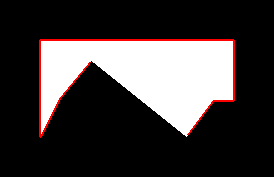
\includegraphics[scale=0.45]{figures/chapter9/constrained-elastica/curve-2/composite-fixed-pixels.png}
}
\subfloat[Curve-2]{
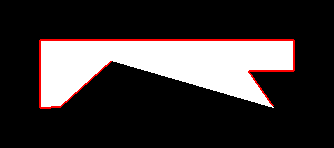
\includegraphics[scale=0.45]{figures/chapter9/constrained-elastica/curve-3/composite-fixed-pixels.png}
}
\subfloat[Too large radius]{
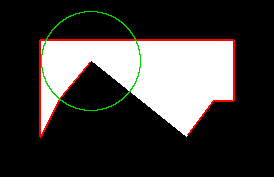
\includegraphics[scale=0.45]{figures/chapter9/constrained-elastica/curve-2/too-big-radius.png}
}
\caption{\daniel{\textbf{Constrained elastica curves and radius value}}. The underlying shapes of Curve-1 and Curve-2 for constrained elastica experiments are shown in figures (a) and (b). Pixels in red are forced to persist in the solution. In figure (c), an example of a too large radius value $(50)$, larger than the shape reach.}
\label{ch9:fig:constrained-elastica-underlying-curve-shapes}
\end{figure}

\begin{figure}
\center
\hspace*{-1cm}
\begin{tabular}{cccc}
\multicolumn{2}{c}{LocalSearch} & \multicolumn{2}{c}{GraphFlow}\\
$\alpha=0.002$ & $\alpha=0.0002$ & $\alpha=0.002$ & $\alpha=0.0002$\\
\subfloat[\label{ch9:fig:results-constrained-elastica-general-a}]{
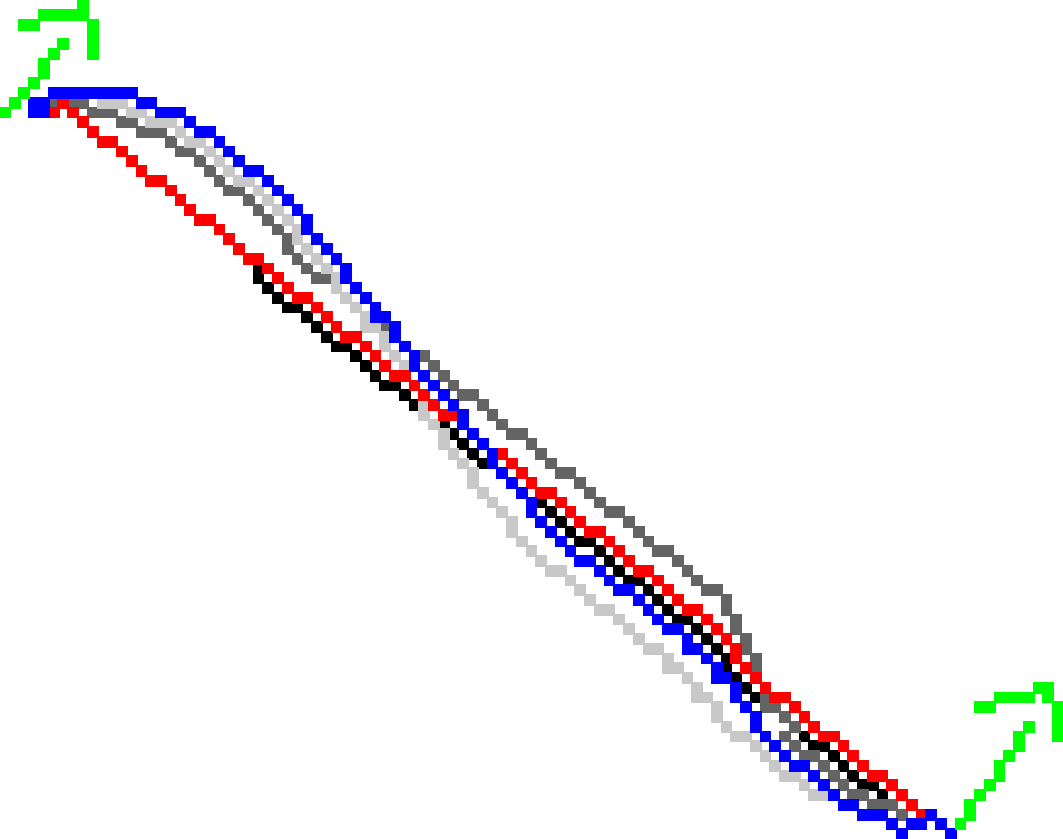
\includegraphics[scale=0.2]{figures/chapter9/constrained-elastica/localsearch/curve-2/len_pen-0.002/radius-7/nc-4/h1.0/summary.pdf}} &
\subfloat[\label{ch9:fig:results-constrained-elastica-general-b}]{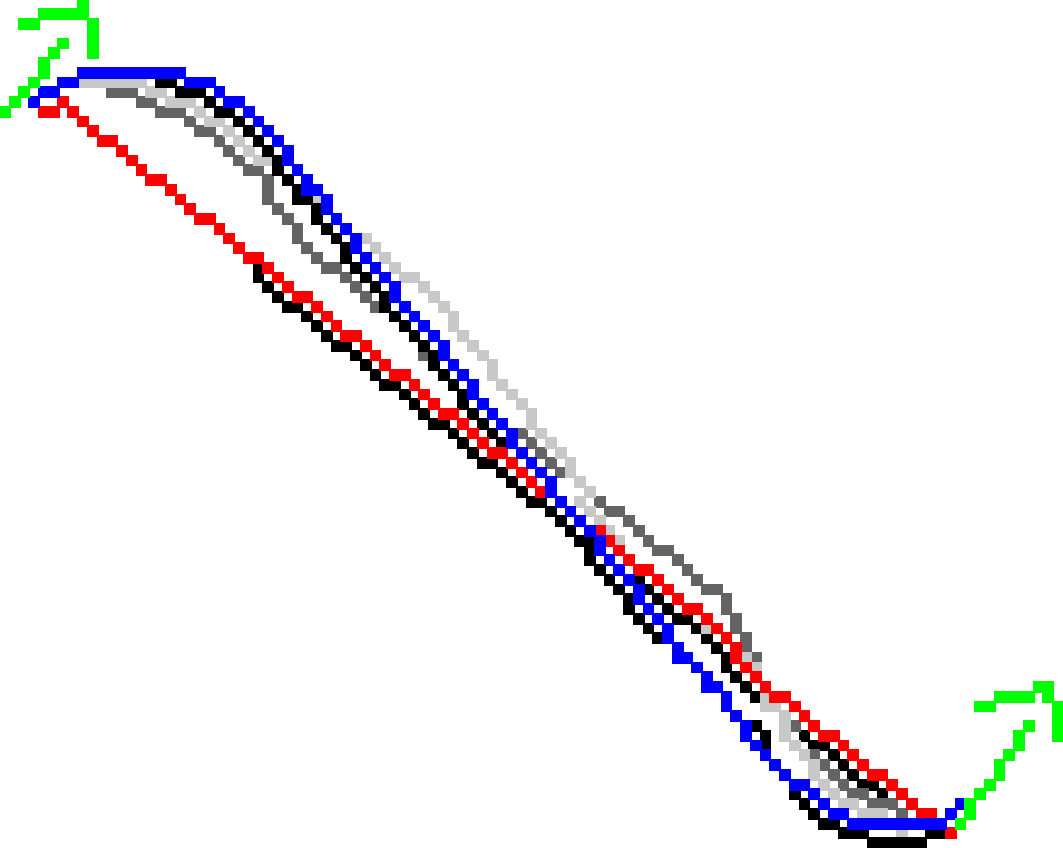
\includegraphics[scale=0.2]{figures/chapter9/constrained-elastica/localsearch/curve-2/len_pen-0.0002/radius-7/nc-4/h1.0/summary.pdf}} &
\subfloat[\label{ch9:fig:results-constrained-elastica-general-c}]{\includegraphics[scale=0.2]{figures/chapter9/constrained-elastica/graphflow/curve-2/len_pen-0.002/radius-7/N-1/h1.0/summary.pdf}} &
\subfloat[\label{ch9:fig:results-constrained-elastica-general-d}]{\includegraphics[scale=0.2]{figures/chapter9/constrained-elastica/graphflow/curve-2/len_pen-0.0002/radius-7/N-1/h1.0/summary.pdf}}\\
\subfloat[\label{ch9:fig:results-constrained-elastica-general-e}]{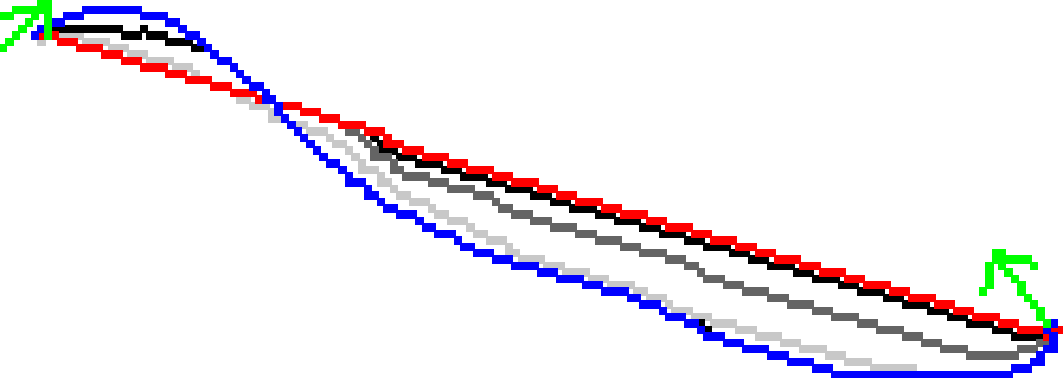
\includegraphics[scale=0.2]{figures/chapter9/constrained-elastica/localsearch/curve-3/len_pen-0.002/radius-7/nc-4/h1.0/summary.pdf}} &
\subfloat[\label{ch9:fig:results-constrained-elastica-general-f}]{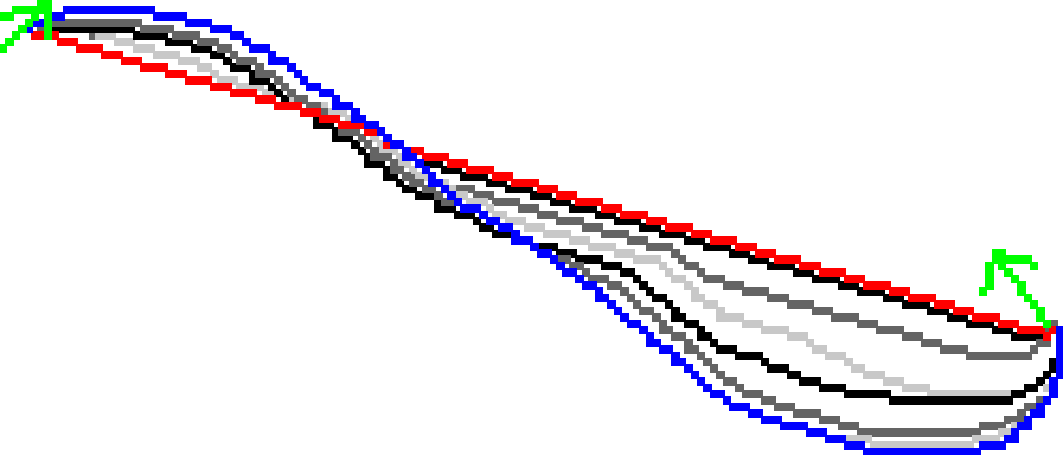
\includegraphics[scale=0.2]{figures/chapter9/constrained-elastica/localsearch/curve-3/len_pen-0.0002/radius-7/nc-4/h1.0/summary.pdf}} &
\subfloat[\label{ch9:fig:results-constrained-elastica-general-g}]{\includegraphics[scale=0.2]{figures/chapter9/constrained-elastica/graphflow/curve-3/len_pen-0.002/radius-7/N-1/h1.0/summary.pdf}} &
\subfloat[\label{ch9:fig:results-constrained-elastica-general-h}]{\includegraphics[scale=0.2]{figures/chapter9/constrained-elastica/graphflow/curve-3/len_pen-0.0002/radius-7/N-1/h1.0/summary.pdf}}\\
\subfloat[\label{ch9:fig:results-constrained-elastica-general-i}]{\includegraphics[scale=0.2]{figures/chapter9/constrained-elastica/localsearch/flower-1/len_pen-0.002/radius-7/nc-4/h1.0/summary.pdf}} &
\subfloat[\label{ch9:fig:results-constrained-elastica-general-j}]{\includegraphics[scale=0.2]{figures/chapter9/constrained-elastica/localsearch/flower-1/len_pen-0.0002/radius-7/nc-4/h1.0/summary.pdf}} &
\subfloat[\label{ch9:fig:results-constrained-elastica-general-k}]{\includegraphics[scale=0.2]{figures/chapter9/constrained-elastica/graphflow/flower-1/len_pen-0.002/radius-7/N-1/h1.0/summary.pdf}} &
\subfloat[\label{ch9:fig:results-constrained-elastica-general-l}]{\includegraphics[scale=0.2]{figures/chapter9/constrained-elastica/graphflow/flower-1/len_pen-0.0002/radius-7/N-1/h1.0/summary.pdf}}\\
\subfloat[\label{ch9:fig:results-constrained-elastica-general-m}]{\includegraphics[scale=0.2]{figures/chapter9/constrained-elastica/localsearch/flower-2/len_pen-0.002/radius-7/nc-4/h1.0/summary.pdf}} &
\subfloat[\label{ch9:fig:results-constrained-elastica-general-n}]{\includegraphics[scale=0.2]{figures/chapter9/constrained-elastica/localsearch/flower-2/len_pen-0.0002/radius-7/nc-4/h1.0/summary.pdf}} &
\subfloat[\label{ch9:fig:results-constrained-elastica-general-o}]{\includegraphics[scale=0.2]{figures/chapter9/constrained-elastica/graphflow/flower-2/len_pen-0.002/radius-7/N-1/h1.0/summary.pdf}} &
\subfloat[\label{ch9:fig:results-constrained-elastica-general-p}]{\includegraphics[scale=0.2]{figures/chapter9/constrained-elastica/graphflow/flower-2/len_pen-0.0002/radius-7/N-1/h1.0/summary.pdf}}\\
\end{tabular}
\caption{\daniel{\textbf{Results of Exp-$\alpha$ for the constrained elastica.}} Initial contour is colored in red and final contour is colored in blue. The green pixels indicates pixels forced to persist in the final contour, or a forced orientation. Curves are drawn every $10$ iterations.}
\label{ch9:fig:results-constrained-elastica-general}
\end{figure}

\begin{figure}
\center
\begin{tabular}{cccc}
\multicolumn{2}{c}{LocalSearch} & \multicolumn{2}{c}{GraphFlow}\\
$r=15$ & $r=50$ & $r=15$ & $r=50$\\

\subfloat[\label{ch9:fig:results-constrained-elastica-radius-a}]{
\includegraphics[scale=0.2]{figures/chapter9/constrained-elastica/localsearch/curve-2/len_pen-0.002/radius-15/nc-4/h1.0/summary.pdf}} &
\subfloat[\label{ch9:fig:results-constrained-elastica-radius-b}]{\includegraphics[scale=0.2]{figures/chapter9/constrained-elastica/localsearch/curve-2/len_pen-0.002/radius-50/nc-4/h1.0/summary.pdf}} &
\subfloat[\label{ch9:fig:results-constrained-elastica-radius-c}]{\includegraphics[scale=0.2]{figures/chapter9/constrained-elastica/graphflow/curve-2/len_pen-0.002/radius-15/N-1/h1.0/summary.pdf}} &
\subfloat[\label{ch9:fig:results-constrained-elastica-radius-d}]{\includegraphics[scale=0.2]{figures/chapter9/constrained-elastica/graphflow/curve-2/len_pen-0.002/radius-50/N-1/h1.0/summary.pdf}}\\

\subfloat[\label{ch9:fig:results-constrained-elastica-radius-e}]{\includegraphics[scale=0.2]{figures/chapter9/constrained-elastica/localsearch/curve-3/len_pen-0.002/radius-15/nc-4/h1.0/summary.pdf}} &
\subfloat[\label{ch9:fig:results-constrained-elastica-radius-f}]{\includegraphics[scale=0.2]{figures/chapter9/constrained-elastica/localsearch/curve-3/len_pen-0.002/radius-50/nc-4/h1.0/summary.pdf}} &
\subfloat[\label{ch9:fig:results-constrained-elastica-radius-g}]{\includegraphics[scale=0.2]{figures/chapter9/constrained-elastica/graphflow/curve-3/len_pen-0.002/radius-15/N-1/h1.0/summary.pdf}} &
\subfloat[\label{ch9:fig:results-constrained-elastica-radius-h}]{\includegraphics[scale=0.2]{figures/chapter9/constrained-elastica/graphflow/curve-3/len_pen-0.002/radius-50/N-1/h1.0/summary.pdf}}\\

\subfloat[\label{ch9:fig:results-constrained-elastica-radius-i}]{\includegraphics[scale=0.2]{figures/chapter9/constrained-elastica/localsearch/flower-1/len_pen-0.002/radius-15/nc-4/h1.0/summary.pdf}} &
\subfloat[\label{ch9:fig:results-constrained-elastica-radius-j}]{\includegraphics[scale=0.2]{figures/chapter9/constrained-elastica/localsearch/flower-1/len_pen-0.002/radius-50/nc-4/h1.0/summary.pdf}} &
\subfloat[\label{ch9:fig:results-constrained-elastica-radius-k}]{\includegraphics[scale=0.2]{figures/chapter9/constrained-elastica/graphflow/flower-1/len_pen-0.002/radius-15/N-1/h1.0/summary.pdf}} &
\subfloat[\label{ch9:fig:results-constrained-elastica-radius-l}]{\includegraphics[scale=0.2]{figures/chapter9/constrained-elastica/graphflow/flower-1/len_pen-0.002/radius-50/N-1/h1.0/summary.pdf}}\\

\subfloat[\label{ch9:fig:results-constrained-elastica-radius-m}]{\includegraphics[scale=0.2]{figures/chapter9/constrained-elastica/localsearch/flower-2/len_pen-0.002/radius-15/nc-4/h1.0/summary.pdf}} &
\subfloat[\label{ch9:fig:results-constrained-elastica-radius-n}]{\includegraphics[scale=0.2]{figures/chapter9/constrained-elastica/localsearch/flower-2/len_pen-0.002/radius-50/nc-4/h1.0/summary.pdf}} &
\subfloat[\label{ch9:fig:results-constrained-elastica-radius-o}]{\includegraphics[scale=0.2]{figures/chapter9/constrained-elastica/graphflow/flower-2/len_pen-0.002/radius-15/N-1/h1.0/summary.pdf}} &
\subfloat[\label{ch9:fig:results-constrained-elastica-radius-p}]{\includegraphics[scale=0.2]{figures/chapter9/constrained-elastica/graphflow/flower-2/len_pen-0.002/radius-50/N-1/h1.0/summary.pdf}}\\


\end{tabular}
\caption{\daniel{\textbf{Results of Exp-Radius for the constrained elastica.}} Initial contour is colored in red and final contour is colored in blue. The green pixels indicates pixels forced to persist in the final contour, or a forced orientation. Curves are drawn every $10$ iterations.}
\label{ch9:fig:results-constrained-elastica-radius}
\end{figure}


\begin{figure}
\center
\captionsetup{type=table}
\begin{tabular}{|l|c|c|c|c|c|}
\hline
& Pixels (initial shape) & LocalSearch & GraphFlow \\
\hline
Curve-1 & 12306 & 4.7s/it & 1s/it\\
Curve-2 & 11527 & 6.2s/it & 1s/it\\
Flower-1  & 7481 & 4.5s/it & 0.3s/it \\
Flower-2 & 7481 & 2.5s/it & 0.21s/it\\
\hline
\end{tabular}
\caption{\daniel{\textbf{Running time and input size of the Exp-$\alpha$ experiment for the constrained elastica.}} The pixels columns is with respect the number of pixels in the shape. In the case of the curves, it is with respect to the underlying shapes of~\cref{ch9:fig:constrained-elastica-underlying-curve-shapes}}
\label{ch9:tab:rtime-constrained-elastica-general} 
\end{figure}

%The parameters used in the comparison are listed in table~\cref{} and the running times in table~\cref{}. The results are displayed in figures~\cref{} and~\cref{}, one for each value of $\alpha$. 

\section{Image segmentation}

The FlipFlow,BalanceFlow and GraphFlow can be extended to do image segmentation. In this section we show the results of several experiments that illustrates the influence of each of the weight parameters (length,curvature,data) and the radius of the estimation disk in the produced segmentation. In the last section we compare our results with the linear programming model for squared curvature regularization SLCR~\cite{schoenemann09linear}. 

All three models (FF,BF,GF) need an initial segmentation as input. This segmentation is given by the graph cut algorithm~\cite{boykov01graphcut}.~\cref{ch9:tab:image-segmentation-parameters-summary} lists the parameters configuration for each experiment and~\cref{ch9:tab:rtime-image-segmentation-general} summarizes their running times. 

The experiments are divided in two sections. In the first, we study the influence of each parameter in the produced segmentation and in the second we compare our results with those produced by SLCR. For the same reason described in the previous section, the grid step in all experiments is set to $h=1.0$.


\begin{table}
\small
\centering
\begin{tabular}{|c|c|c|c|c|c|c|c|c|c|c|c|c|}
\cline{8-13}
\multicolumn{7}{c|}{} & \multicolumn{2}{|c|}{FF,BF} & \multicolumn{4}{|c|}{GF}\\
\hline
Experiment & $maxIt$ & $vRadius$ & $bRadius$ & $h$ & $\alpha$ & $\beta$  & $\gamma$ & $d$ & $a$ & $n$ & $\gamma_r$ & $\gamma_b$ \\
\hline
\multirow{3}{*}{Exp-$\alpha$} & \multirow{3}{*}{$200$} & \multirow{3}{*}{$7$} & \multirow{3}{*}{$7$} & \multirow{3}{*}{$1.0$} & $0$ & \multirow{3}{*}{$0$} & \multirow{3}{*}{$1$} & \multirow{3}{*}{$0$} & \multirow{3}{*}{$2$} & \multirow{3}{*}{$2$} & \multirow{3}{*}{$1$} & \multirow{3}{*}{$0$} \\
&  & & & & $0.5$ & & & & & & &\\
&  & & & & $3.0$ & & & & & & &\\
\hline
\multirow{3}{*}{Exp-$\beta$} & \multirow{3}{*}{$200$} & \multirow{3}{*}{$7$} & \multirow{3}{*}{$7$} & \multirow{3}{*}{$1.0$} & \multirow{3}{*}{$0$} & $0.1$ & \multirow{3}{*}{$1$} & \multirow{3}{*}{$0$} & \multirow{3}{*}{$2$} & \multirow{3}{*}{$2$} & \multirow{3}{*}{$1$} & \multirow{3}{*}{$1$} \\
&  & & & & & $1$ & & & & & &\\
&  & & & & & $2$ & & & & & &\\
\hline
\multirow{3}{*}{Exp-$\gamma$} & \multirow{3}{*}{$200$} & \multirow{3}{*}{$7$} & \multirow{3}{*}{$7$} & \multirow{3}{*}{$1.0$} & \multirow{3}{*}{$0$} & \multirow{3}{*}{$1$} & $1$ & \multirow{3}{*}{$0$} & \multirow{3}{*}{$2$} & \multirow{3}{*}{$2$} & $1$ & $1$ \\
&  & & & & & & $2$ & & & & $2$ & $2$\\
&  & & & & & & $5$ & & & & $5$ & $5$\\
\hline
\multirow{3}{*}{Exp-$rbRadius$} & \multirow{3}{*}{$200$} & $3$ & $3$ & \multirow{3}{*}{$1.0$} &  \multirow{3}{*}{$0$} & \multirow{3}{*}{$3$} & \multirow{3}{*}{$1$} & \multirow{3}{*}{$0$} & \multirow{3}{*}{$2$} & \multirow{3}{*}{$2$} & \multirow{3}{*}{$1$} & \multirow{3}{*}{$1$} \\
&  & $7$ & $7$ & & & & & & & & & \\
&  & $12$ & $12$ & & & & & & & & & \\
\hline
\end{tabular}
\caption{\daniel{\textbf{Parameter settings for the image segmentation experiments.}} The headers FF,BF,GF identifies parameters that are exclusive of FlipFlow, BalanceFlow and GraphFlow models, respectively.}
\label{ch9:tab:image-segmentation-parameters-summary}
\end{table}


\begin{table}
\small
\centering
\begin{tabular}{|c|c|c|c|c|c|c|c|c|c|c|c|c|}
\hline
\multicolumn{13}{|c|}{Exp-Comparison}\\
\hline
Model & $maxIt$ & $vRadius$ & $bRadius$ & $h$ & $\alpha$ & $\beta (\lambda)$  & $\gamma$ & $d$ & $a$ & $ob$ & $\gamma_r$ & $\gamma_b$ \\
\hline
FF,BF & $200$ & $7$ & $7$ & $1.0$ & $0.5$ & $1.0$ & $1.0$ & $0$ & - & - & - & -\\
\hline
GF & $200$ & $7$ & $7$ & $1.0$ & $0.0002$ & $1.0$ & - & - & $2$ & $2$ & $3$ & $3$\\
\hline
SCLR & - & - & - & - & - & $2.0$ & $1.0$ & - & - & - & - & -\\
\hline
\end{tabular}
\caption{\daniel{\textbf{Parameter settings for the comparison experiments.}} The $\beta$ parameter in FF,BF,GF corresponds to the $\lambda$ parameter in SCLR.}
\label{ch9:tab:image-segmentation-comparison-summary}
\end{table}

\begin{figure}
\center
\captionsetup{type=table}
\begin{tabular}{|c|c|c|c|}
\hline
\multicolumn{4}{|c|}{Exp-Comparison Running time}\\
\hline
Model & Minimum & Maximum & Average \\
\hline
FlipFlow & 60s & 297s & 156s\\
BalanceFlow & 37s & 184s & 93.7s\\
GraphFlow & 11s & 150s & 75s\\
SLCR & 2.87min & 52.24min & 18.4min\\
\hline
\end{tabular}
\caption{Running time and input size of Exp-$bRadius$ for the image segmentation problem and $bRadius=7$.}
\label{ch9:tab:rtime-image-segmentation-general} 
\end{figure}

\subsection{Influence of parameters}
The models offer parameters to control the relative weight of length $(\alpha)$, curvature $(\beta)$ and data ($\gamma,\gamma _r, \gamma _b$). We recall that FF and BF accept a single regional parameter $\gamma$ for data, while GF accepts $\gamma _r$ to ponderate a regional term and $\gamma _b$ to weight a boundary term. The graph cut input and its result are shown in~\cref{ch9:fig:grabcut-input-image-segmentation}. The experiment results are displayed in~\cref{ch9:fig:exp-alpha-image-segmentation,ch9:fig:exp-beta-image-segmentation,ch9:fig:exp-gamma-image-segmentation,ch9:fig:exp-radius-image-segmentation}. 

The FlipFlow and BalanceFlow present similar results for all experiments, as expected. The Exp-$\alpha$ experiment regularizes only length, and we can observe that the segmentations produced by all three models tend to be staircased. We remark that in the GF model, length penalization is not present in the cost function of the candidate graph, but only in the validation function. In particular, we need  a $a$-probe set with $a>0$ so that length penalization has an influence in the produced segmentation.

In experiment Exp-$\beta$, we vary the squared curvature weight coefficient. We observe in~\cref{ch9:fig:exp-beta-image-segmentation} that the produced segmentation smooths out for increasing values of $\beta$. We recall that the shrink/growing behavior in the GF is controlled by the value of $\alpha$. The FF and BF grow in concavities, but unless a local optimum is found, they tend to shrink.

The models' response for the variation of data term is shown in~\cref{ch9:fig:exp-gamma-image-segmentation}. A higher value of $\gamma$ tends to produce results similar to the initial segmentation given by graph cut, i.e., with almost no length or curvature regularization.

Finally, Exp-$bRadius$ illustrates how the choice of the estimation disk radius influences the segmentation. In~\cref{ch9:fig:exp-radius-image-segmentation} we observe that a small radius results in contours with sharp changes of angle (first row), a consequence of the limited number of different estimations that can be given by a disk of small radius. As the radius increase, a richer variation of estimations is possible, and we have smoother contours (second-row). However, a big radius may omit important details of the object, as the coala's ears in the last row of~\cref{ch9:fig:exp-radius-image-segmentation}. That suggests that a multiradius approach may deliver improved segmentations.


\begin{figure}
\centering
\begin{tabular}{cc}
\includegraphics[scale=0.4]{figures/chapter9/segmentation/seeds.png} &
\includegraphics[scale=0.4]{figures/chapter9/segmentation/gc-seg.png}
\end{tabular}
\caption{Foreground (green) and background (blue) seeds are shown in the left and the resulting graph cut segmentation in the right.}
\label{ch9:fig:grabcut-input-image-segmentation}
\end{figure}

\newcommand\expAlphaFF[2]{figures/chapter9/segmentation/exp-alpha/#1/h-1.0/dalpha-False/neigh-0/alpha-#2/beta-0.0/lb-1.0/lr-1.0/coala/corrected_seg.png}
\newcommand\expAlphaGF[2]{figures/chapter9/segmentation/exp-alpha/#1/h-1.0/dalpha-False/neigh-2/alpha-#2/beta-0.0/lb-0.0/lr-1.0/coala/corrected_seg.png}


\begin{figure}
\centering
\subfloat[$\alpha=0.0$]{
\begin{tabular}{ccc}
FlipFlow & BalanceFlow & GraphFlow\\
\includegraphics[scale=0.38]{\expAlphaFF{flipseg}{0.0}} &
\includegraphics[scale=0.38]{\expAlphaFF{balanceseg}{0.0}} &
\includegraphics[scale=0.38]{\expAlphaGF{graphseg}{0.0}}
\end{tabular}} \\

\subfloat[$\alpha=0.5$]{
\begin{tabular}{ccc}
\includegraphics[scale=0.38]{\expAlphaFF{flipseg}{0.5}} &
\includegraphics[scale=0.38]{\expAlphaFF{balanceseg}{0.5}} &
\includegraphics[scale=0.38]{\expAlphaGF{graphseg}{0.5}}\\
\end{tabular}} \\

\subfloat[$\alpha=3.0$]{
\begin{tabular}{ccc}
\includegraphics[scale=0.38]{\expAlphaFF{flipseg}{3.0}} &
\includegraphics[scale=0.38]{\expAlphaFF{balanceseg}{3.0}} &
\includegraphics[scale=0.38]{\expAlphaGF{graphseg}{3.0}}
\end{tabular}}
\caption{\daniel{\textbf{Results of Exp-$\alpha$ for segmentation.}}}
\label{ch9:fig:exp-alpha-image-segmentation}
\end{figure}


\newcommand\expBetaFF[2]{figures/chapter9/segmentation/exp-beta/#1/h-1.0/dalpha-False/neigh-0/alpha-0.0/beta-#2/lb-1.0/lr-1.0/coala/corrected_seg.png}
\newcommand\expBetaGF[2]{figures/chapter9/segmentation/exp-beta/#1/h-1.0/dalpha-False/neigh-2/alpha-0.0/beta-#2/lb-1.0/lr-1.0/coala/corrected_seg.png}

\begin{figure}
\centering
\subfloat[$\beta=0.1$]{
\begin{tabular}{ccc}
FlipFlow & BalanceFlow & GraphFlow\\
\includegraphics[scale=0.38]{\expBetaFF{flipseg}{0.1}} &
\includegraphics[scale=0.38]{\expBetaFF{balanceseg}{0.1}} &
\includegraphics[scale=0.38]{\expBetaGF{graphseg}{0.1}}
\end{tabular}}\\

\subfloat[$\beta=1.0$]{
\begin{tabular}{ccc}
\includegraphics[scale=0.38]{\expBetaFF{flipseg}{1.0}} &
\includegraphics[scale=0.38]{\expBetaFF{balanceseg}{1.0}} &
\includegraphics[scale=0.38]{\expBetaGF{graphseg}{1.0}}
\end{tabular}}\\

\subfloat[$\beta=2.0$]{
\begin{tabular}{ccc}
\includegraphics[scale=0.38]{\expBetaFF{flipseg}{2.0}} &
\includegraphics[scale=0.38]{\expBetaFF{balanceseg}{2.0}} &
\includegraphics[scale=0.38]{\expBetaGF{graphseg}{2.0}}
\end{tabular}}
\caption{\daniel{\textbf{Results of Exp-$\beta$ for segmentation.}}}
\label{ch9:fig:exp-beta-image-segmentation}
\end{figure}

\newcommand\expGamaFF[2]{figures/chapter9/segmentation/exp-gamma/#1/h-1.0/dalpha-False/neigh-0/alpha-0.0/beta-1.0/lb-#2/lr-#2/coala/corrected_seg.png}
\newcommand\expGamaGF[2]{figures/chapter9/segmentation/exp-gamma/#1/h-1.0/dalpha-False/neigh-2/alpha-0.0/beta-1.0/lb-#2/lr-#2/coala/corrected_seg.png}

\begin{figure}
\centering
\subfloat[$\gamma =1.0$]{
\begin{tabular}{ccc}
FlipFlow & BalanceFlow & GraphFlow\\
\includegraphics[scale=0.38]{\expGamaFF{flipseg}{1.0}} &
\includegraphics[scale=0.38]{\expGamaFF{balanceseg}{1.0}} &
\includegraphics[scale=0.38]{\expGamaGF{graphseg}{1.0}}
\end{tabular}} \\

\subfloat[$\gamma =2.0$]{
\begin{tabular}{ccc}
\includegraphics[scale=0.38]{\expGamaFF{flipseg}{2.0}} &
\includegraphics[scale=0.38]{\expGamaFF{balanceseg}{2.0}} &
\includegraphics[scale=0.38]{\expGamaGF{graphseg}{2.0}}
\end{tabular}}\\

\subfloat[$\gamma =5.0$]{ 
\begin{tabular}{ccc}
\includegraphics[scale=0.38]{\expGamaFF{flipseg}{5.0}} &
\includegraphics[scale=0.38]{\expGamaFF{balanceseg}{5.0}} &
\includegraphics[scale=0.38]{\expGamaGF{graphseg}{5.0}}
\end{tabular}}
\caption{\daniel{\textbf{Results of Exp-$\gamma$ for segmentation.}}}
\label{ch9:fig:exp-gamma-image-segmentation}
\end{figure}


\newcommand\expRadiusFF[2]{figures/chapter9/segmentation/exp-radius/#1/h-1.0/alpha-0.0/beta-3.0/gamma-1.0/radius-#2/corrected-seg.png}
\newcommand\expRadiusGF[2]{figures/chapter9/segmentation/exp-radius/#1/h-1.0/alpha-0.0/beta-3.0/gamma-1.0/radius-#2/corrected-seg.png}

\begin{figure}
\centering
\subfloat[$r=3$]{
\begin{tabular}{ccc}
FlipFlow & BalanceFlow & GraphFlow\\ 
\includegraphics[scale=0.38]{\expRadiusFF{flipseg}{3}} &
\includegraphics[scale=0.38]{\expRadiusFF{balanceseg}{3}} &
\includegraphics[scale=0.38]{\expRadiusGF{graphseg}{3}}
\end{tabular}}

\subfloat[$r=7$]{
\begin{tabular}{ccc}
\includegraphics[scale=0.38]{\expRadiusFF{flipseg}{7}} &
\includegraphics[scale=0.38]{\expRadiusFF{balanceseg}{7}} &
\includegraphics[scale=0.38]{\expRadiusGF{graphseg}{7}}
\end{tabular}}

\subfloat[$r=12$]{
\begin{tabular}{ccc}
\includegraphics[scale=0.38]{\expRadiusFF{flipseg}{12}} &
\includegraphics[scale=0.38]{\expRadiusFF{balanceseg}{12}} &
\includegraphics[scale=0.38]{\expRadiusGF{graphseg}{12}}
\end{tabular}}

\caption{\daniel{\textbf{Results of Exp-$Radius$ for segmentation.}}}
\label{ch9:fig:exp-radius-image-segmentation}
\end{figure}

\subsection{Comparison}

In~\cref{ch9:fig:exp-comparison-image-segmentation-1,ch9:fig:exp-comparison-image-segmentation-2,ch9:fig:exp-comparison-image-segmentation-3,ch9:fig:exp-comparison-image-segmentation-4}, we show the segmentation results of several images for the three models developed in this thesis, the SLCR and graph cut models. We opt to set the same parameters in all instances, although a better segmentation could be obtained by setting them separately.

The curvature regularization in the FF,BF models are well perceived in the airplane, camel and man-in-white pictures, but those models are not able to correctly segment the brown-snake in~\cref{ch9:fig:exp-comparison-image-segmentation-4}. They also have a hard time to segment the birds in~\cref{ch9:fig:exp-comparison-image-segmentation-2} due to the object large curvature range. Nonetheless, they correctly segmented the green-snake in~\cref{ch9:fig:exp-comparison-image-segmentation-3} while the graph cut return three disconnected components.

For the chosen parameters, the GraphFlow did not evolve the initial graph cut segmentation to much, except for the brown-snake in~\cref{ch9:fig:exp-comparison-image-segmentation-4}, for which GF and SLCR presented the best segmentation. However, the GF has the second lowest running time among the five models.

The SLCR tends to oversegment, notably in the man-in-white and the camel pictures. We observe that the contours present sharp turns due to the low precision of the curvature estimator. The precision could be improved by increasing the pixels connectivity (set to $8$), but this is likely to follow an increase in running time, which is already the highest between the models tested.





\newcommand\segComparisonGF[2]{figures/chapter9/segmentation/comparison/#1/#2/alpha-0.0002/beta-1.0/gamma-3.0/radius-7}
\newcommand\segComparisonFF[2]{figures/chapter9/segmentation/comparison/#1/#2/alpha-0.5/beta-1.0/gamma-3.0/radius-7}
\newcommand\segComparisonScho[2]{figures/chapter9/segmentation/comparison/#1/lambda-2.0/gamma-1.0/#2}

\newcommand\compTable[5]{
	\begin{figure}
	\center
	\setlength{\tabcolsep}{1pt}
	\begin{tabular}{m{0.25cm}ccc}
	\rotatebox{90}{Graph cut} & 
	\figTable{0.32}{\segComparisonFF{flipseg}{#1}/gc-seg.png} & 
	\figTable{0.32}{\segComparisonFF{flipseg}{#2}/gc-seg.png} & 
	\figTable{0.32}{\segComparisonFF{flipseg}{#3}/gc-seg.png} \\[6em]
	
	\rotatebox{90}{SCLR} & 
	\figTable{0.32}{\segComparisonScho{schoenemann}{#1}/#1.png} & 
	\figTable{0.32}{\segComparisonScho{schoenemann}{#2}/#2.png} & 
	\figTable{0.32}{\segComparisonScho{schoenemann}{#3}/#3.png}\\[6em]
	
	\rotatebox{90}{FlipFlow} & 
	\figTable{0.32}{\segComparisonFF{flipseg}{#1}/corrected-seg.png} & 
	\figTable{0.32}{\segComparisonFF{flipseg}{#2}/corrected-seg.png} & 
	\figTable{0.32}{\segComparisonFF{flipseg}{#3}/corrected-seg.png} \\[6em]
	
	\rotatebox{90}{BalanceFlow} & 
	\figTable{0.32}{\segComparisonFF{balanceseg}{#1}/corrected-seg.png} & 
	\figTable{0.32}{\segComparisonFF{balanceseg}{#2}/corrected-seg.png} & 
	\figTable{0.32}{\segComparisonFF{balanceseg}{#3}/corrected-seg.png}\\[6em]
	
	\rotatebox{90}{GraphFlow} & 
	\figTable{0.32}{\segComparisonGF{graphseg}{#1}/corrected-seg.png} & 
	\figTable{0.32}{\segComparisonGF{graphseg}{#2}/corrected-seg.png} & 
	\figTable{0.32}{\segComparisonGF{graphseg}{#3}/corrected-seg.png}
	\end{tabular}
	\caption{#4}
	\label{#5}
	\end{figure}
}


\compTable{airplane}{kite-surf}{mans-music}{\daniel{\textbf{Segmentation results comparison set 1}}}{ch9:fig:exp-comparison-image-segmentation-1}
\compTable{birds}{brown-snake}{tiger}{\daniel{\textbf{Segmentation results comparison set 2.}}}{ch9:fig:exp-comparison-image-segmentation-2}
\compTable{camel}{green-snake}{peacock}{\daniel{\textbf{Segmentation results comparison set 3.}}}{ch9:fig:exp-comparison-image-segmentation-3}
%\compTable{long-snake}{mushroom}{statues}{Comparison 4}{ch9:fig:exp-comparison-image-segmentation-4}


\afterpage{%
    \clearpage% Flush earlier floats (otherwise order might not be correct)
    \thispagestyle{empty}% empty page style (?)
    \begin{landscape}% Landscape page

	\begin{figure}
	\center
	\begin{tabular}{ccccc}
	Graph cut & SLCR & FlipFlow & BalanceFlow & GraphFlow\\
	\figTable{0.32}{\segComparisonFF{flipseg}{long-snake}/gc-seg.png} & 
	\figTable{0.32}{\segComparisonScho{schoenemann}{long-snake}/long-snake.png} & 
	\figTable{0.32}{\segComparisonFF{flipseg}{long-snake}/corrected-seg.png} & 		
	\figTable{0.32}{\segComparisonFF{balanceseg}{long-snake}/corrected-seg.png} & 			
	\figTable{0.32}{\segComparisonGF{graphseg}{long-snake}/corrected-seg.png} \\[10em]	
	
	\figTable{0.32}{\segComparisonFF{flipseg}{statues}/gc-seg.png} & 
	\figTable{0.32}{\segComparisonScho{schoenemann}{statues}/statues.png} & 
	\figTable{0.32}{\segComparisonFF{flipseg}{statues}/corrected-seg.png} & 		
	\figTable{0.32}{\segComparisonFF{balanceseg}{statues}/corrected-seg.png} & 			
	\figTable{0.32}{\segComparisonGF{graphseg}{statues}/corrected-seg.png}
	
	
	\end{tabular}
	\caption{\daniel{\textbf{Segmentation results comparison set 4}}}
	\label{ch9:fig:exp-comparison-image-segmentation-4}
	\end{figure}

    \end{landscape}
    \clearpage% Flush page
}



\section{Conclusion}

All the four models described in this thesis can be used to produce shapes of lower digital elastica. Moreover, the FlipFlow,BalanceFlow and GraphFlow can be extended to do image segmentation with curvature regularization. In particular, the GraphFlow is a straightforward extension of the standard graph cut model, which originally did not implement geometric regularization, and presents lower running times than FF and BF. Additionally, we observe that the GraphFlow can recover the completion property associated to the squared curvature regularization in some occasions. Finally, our models are competitive with the SLCR segmentation algorithm that employs curvature regularization.




